% !TEX root = ../main_without_quantization.tex
\chapter{Methodology}

In this chapter we present our methodology to find compressed transformer architectures within a budget. The aim is to formalize the notion of allocation-aware compression into a pipeline that identifies a candidate compression, applies budget constraints, compares candidates before recovery, searches the feasible space, then finally finetunes the candidate.

The presentation uses encoder structured pruning as the main running example because it is the most detailed setting in the work. The same methodology also applies to decoder compression, where the candidate representation changes according to the compression family. In both cases, the central question is how the available budget should be distributed across the model so that the compressed architecture remains recoverable.

The chapter follows the order of the pipeline. It first defines the search object and the budget constraint, then introduces the pre-recovery ranking signal used to compare candidates. It then presents the evolutionary search procedure and the recovery stage applied after selection.

\clearpage
% !TEX root = ../../main_without_quantization.tex
\section{Candidate Parameterisation}
\label{chap:mask}

This section defines the candidate representation used by the search. A candidate can be seen as a record for the compressed units selected for one architecture, and naturally, its  own form depends on the compression family. In our case, the encoder structured pruning uses binary masks over attention heads and feed-forward neurons, whicj follows the unit granularity used in structured Transformer pruning \citep{michel2022not,xia2022cofi,kurtic2023ziplm} and the decoder compression uses discrete level vectors for layer dropping, quantization, low-rank factorisation, and rank-based recovery. 

The first encoding is the structured-pruning mask used for the encoder experiments in which we will elaborate on in the next point.

\subsection{Encoder Structured-Pruning Encoding}

A candidate architecture is a pair of binary masks
\begin{equation}
\cand = (\Maskh, \Maskn)
\in
\{0,1\}^{\nlayers \times \nheads}
\times
\{0,1\}^{\nlayers \times \nffn}.
\end{equation}
For layer $\ell$, the active attention heads and active feed forward neurons are
\begin{equation}
H_\ell(\cand) = \{h : \Maskh[\ell,h] = 1\},
\qquad
N_\ell(\cand) = \{n : \Maskn[\ell,n] = 1\}.
\end{equation}
The head mask selects all head slices in the attention projections of the Transformer. The neuron mask selects the rows of the first feed forward projection and corresponding columns of the second feed forward projection. Indices for the masks are specified using teacher original coordinates.

For this encoder encoding, the remaining definitions are derived from the same mask pair: structural counts, layer status, and candidate identity.

\subsection{Encoder Structural Counts}

The first derived object is the count vector induced by the two masks, which summarizes the mask for budget control and reporting. At layer $\ell$, summing the binary decisions in each row gives
\begin{align}
a_\ell(\cand) &= \sum_{h=1}^{\nheads} \Maskh[\ell,h], \\
n_\ell(\cand) &= \sum_{n=1}^{\nffn} \Maskn[\ell,n].
\end{align}
In this sense, $a_\ell(\cand)$ records how many attention heads remain in layer $\ell$, whereas $n_\ell(\cand)$ records how many feed forward neurons remain in that same layer. The search keeps these local quantities because cost and behaviour depend on where units are kept.

The global head and neuron counts are then obtained by summing the local counts across depth:
\begin{equation}
A(\cand)=\sum_{\ell=1}^{\nlayers} a_\ell(\cand),
\qquad
N(\cand)=\sum_{\ell=1}^{\nlayers} n_\ell(\cand).
\end{equation}
These totals report candidate size. Since they do not show whether the remaining units are concentrated in a few layers or distributed across many layers, we also track the number of layers that contain at least one active sublayer:
\begin{equation}
L_{\mathrm{act}}(\cand)
=
\sum_{\ell=1}^{\nlayers}
\indic\{a_\ell(\cand) + n_\ell(\cand) > 0\}.
\end{equation}
Finally, the same per-layer counts are used to evaluate the compute budget. Each active head contributes one head cost, and each active feed forward neuron contributes one neuron cost:
\begin{equation}
\macop(\cand)
=
\sum_{\ell=1}^{\nlayers}
\big(a_\ell(\cand)\headcost+n_\ell(\cand)\neuroncost\big),
\end{equation}
where $\headcost$ and $\neuroncost$ are the per head and per neuron costs derived in Section~\ref{chap:cost}.

The pair $(a_\ell,n_\ell)$ also fixes the execution case of layer $\ell$. Table~\ref{tab:layer_statuses} shows how these counts determine the masked forward pass. The search therefore selects both the budget and the computation that remains at each depth.

\begin{table}[h]
\centering
\footnotesize
\setlength{\tabcolsep}{4pt}
\begin{tabularx}{0.86\textwidth}{llX}
\toprule
Condition & Status & Masked forward \\
\midrule
$a_\ell>0,\;n_\ell>0$ & both active &
attention and feed forward execute \\
$a_\ell=0,\;n_\ell>0$ & feed forward only &
attention update is zero; feed forward executes \\
$a_\ell>0,\;n_\ell=0$ & attention only &
attention executes; feed forward update is zero \\
$a_\ell=0,\;n_\ell=0$ & identity &
the layer returns its input \\
\bottomrule
\end{tabularx}
\caption{Layer statuses induced by the structural masks.}
\label{tab:layer_statuses}
\end{table}

This status is utilized whenever a candidate is evaluated. If it has positive counts then it must keep the corresponding sub-layer active, whereas zero counts remove that sub-layer update. Naturally, two candidates with the same global size can behave differently if their active units create different layer statuses. This is why the implementation also needs two levels of candidate description: an exact identity for caching and a coarser signature for population tracking, which is the idea of the next point


\subsection{Encoder Granularity and Candidate Identity}

Neuron choices are grouped for search efficiency. The implementation allocates feed forward neurons in blocks of sixteen. As a direct consequence, $n_\ell(\cand)$ is restricted to multiples of sixteen, except for the zero case. This block size keeps mutation aligned with meaningful cost changes and reduces candidates that differ only by negligible single-neuron moves.

For exact caching, the identity of a candidate is the bit string obtained by concatenating $\Maskh$ and $\Maskn$. Two candidates are identical if and only if this bit string is identical. This key is deliberately fine-grained because it preserves the exact placement of every active unit. For diversity tracking, the search also records the coarser macro signature
\begin{equation}
\sigma(\cand)
=
\big(A(\cand),\,N(\cand),\,L_{\mathrm{act}}(\cand)\big).
\end{equation}
The macro signature loses placement information. Two candidates can have the same total counts and active layer count while assigning compute to different depths, so exact deduplication still uses the full bit string. The macro signature is used only as a population-level descriptor in the search mechanisms described in Section~\ref{chap:detailed_pipeline}.

\subsection{Decoder Compression Encodings}
\label{sec:other_candidate_forms}
\label{sec:decoder_compression_encodings}

The decoder-model searches utilize smaller discrete genomes that point to preset compression options. In this manner, the search space can remain small and the search simply selects feasible level of layer, bit width, rank or recovery. 

\paragraph{Layer drop.}
A candidate is a pair of boolean vectors over the $L$ layers,
\begin{equation}
\cand_{\mathrm{drop}}
=
(d^{\mathrm{attn}}, d^{\mathrm{mlp}})
\in \{0,1\}^{L} \times \{0,1\}^{L},
\end{equation}
where $d^{\mathrm{attn}}_\ell = 1$ marks the attention sub-block of layer $\ell$ as dropped and $d^{\mathrm{mlp}}_\ell = 1$ the feed forward sub-block; a dropped sub-block is replaced by an identity map. The budget fixes the exact number of dropped sub-blocks to $\lfloor s\,(2L) \rfloor$ for a target drop fraction $s$, so every candidate removes the same amount of depth and differs only in placement.

\paragraph{Quantization.}
A candidate assigns a bit-width to each quantizable weight matrix,
\begin{equation}
\cand_{\mathrm{quant}}
=
(b_1, \dots, b_K),
\qquad
b_i \in \mathcal{B},
\end{equation}
where $\mathcal{B}=\{2,2.5,3,4,8\}$ in the experiments. Each value names a pre-quantized version of matrix $i$ that is built offline and then loaded during evaluation. Writing $|W_i|$ for the number of parameters in matrix $i$, the budget caps the size-weighted average bit-width,
\begin{equation}
\sum_{i} b_i\,|W_i| \;\le\; \bar{b} \sum_{i} |W_i|,
\end{equation}
for a target average bit-width $\bar{b}$.

\paragraph{Low-rank factorisation.}
A candidate assigns a retained-rank fraction to each factorised matrix,
\begin{equation}
\cand_{\mathrm{rank}}
=
(\alpha_1, \dots, \alpha_K),
\qquad
\alpha_i \in \mathcal{R},
\end{equation}
where $\mathcal{R}=\{0.05,0.10,0.20,0.35,0.50,0.75\}$ in the experiments. For a matrix of shape $m_i \times n_i$, the retained rank is
\begin{equation}
q_i = \left\lfloor \alpha_i \min(m_i,n_i) \right\rfloor .
\end{equation}
The factorised matrix therefore costs $q_i(m_i+n_i)$ parameters instead of $m_i n_i$. The budget caps the total stored size relative to the dense model,
\begin{equation}
\sum_{i} q_i\,(m_i + n_i) \;\le\; \rho \sum_{i} m_i n_i,
\end{equation}
for a target compression ratio $\rho$.

\paragraph{Rank-based recovery.}
For recovery, a candidate assigns a residual rank to each layer,
\begin{equation}
\cand_{\mathrm{rec}}
=
(r_1, \dots, r_L),
\qquad
0 \le r_\ell \le r_{\mathrm{cap}},
\end{equation}
and the recovered weight of layer $\ell$ adds back the top $r_\ell$ singular components of the residual between the dense and the compressed weight,
\begin{equation}
W_\ell = W^{\mathrm{base}}_\ell + \sum_{i=1}^{r_\ell} \sigma_i\, u_i v_i^\top,
\end{equation}
where $(\sigma_i, u_i, v_i)$ are the residual singular triplets, computed once and reused. The budget caps the average residual rank, $\sum_\ell r_\ell (m_\ell + n_\ell) \le \bar{r} \sum_\ell (m_\ell + n_\ell)$, for a target average rank $\bar{r}$.

Table~\ref{tab:candidate_forms} summarises the encodings used across the encoder and decoder experiments. The rest of the methodology develops the detailed mechanics on the structured-pruning mask because it is the setting that requires explicit head and neuron accounting.

\begin{table}[h]
\centering
\footnotesize
\setlength{\tabcolsep}{4pt}
\begin{tabularx}{\textwidth}{llX}
\toprule
Family & Candidate encoding & Budget constraint \\
\midrule
Encoder structured pruning & head mask $+$ FFN-neuron mask & MAC budget (head and neuron cost) \\
Decoder layer drop & paired boolean vectors $(d^{\mathrm{attn}}, d^{\mathrm{mlp}})$ & exact dropped sub-block count \\
Decoder quantization & per-matrix bit-width $b_i$ & size-weighted average bits $\bar{b}$ \\
Decoder low-rank & per-matrix retained-rank fraction $\alpha_i$ & stored params $\le \rho \sum_i m_i n_i$ \\
Decoder rank recovery & per-layer residual rank $r_\ell$ & average residual rank $\bar{r}$ \\
\bottomrule
\end{tabularx}
\caption{Candidate encodings and budget constraints across the five compression families. The table records what a candidate stores before any search operator, evaluation rule, or recovery step is applied.}
\label{tab:candidate_forms}
\end{table}

% !TEX root = ../../main_without_quantization.tex
\section{Efficiency Budget and Cost Model}
\label{chap:cost}

The binary masks from Section~\ref{chap:mask} indicate which attention heads and which feed-forward neurons are used at each layer. Based on them, the search computes for each candidate a deterministic operation cost, on which feasibility checks, repair and reporting are based. The cost for each candidate is computed with the reference sequence length $\seqlen$.

For one active attention head with head dimension $\dhead$, the mask-dependent projection cost is
\begin{equation}
\headcost = 2 \seqlen \dhid \dhead .
\label{eq:hcost}
\end{equation}
For one active feed-forward neuron, the corresponding cost of the two linear projections is
\begin{equation}
\neuroncost = 2 \seqlen \dhid .
\label{eq:ncost}
\end{equation}

Let $\actl(\cand)$ and $\nactl(\cand)$ denote the active head and neuron counts of layer $\ell$. The layer and candidate costs are
\begin{equation}
\macop_\ell(\cand)
=
\actl(\cand)\headcost+\nactl(\cand)\neuroncost ,
\label{eq:layercost}
\end{equation}
\begin{equation}
\macop(\cand)
=
\sum_{\ell=1}^{\nlayers}\macop_\ell(\cand).
\label{eq:candcost}
\end{equation}
The dense reference cost is
\[
\macdense=\nlayers(\nheads\headcost+\nffn\neuroncost),
\]
and the keep ratio is $\keepratio(\cand)=\macop(\cand)/\macdense$.

The target budget $\budget$ is discrete because head counts are integer and neuron counts are allocated in blocks. A candidate is feasible when its cost lies in the tolerance band
\begin{equation}
(1-\varepsilon)\budget
\le
\macop(\cand)
\le
(1+\varepsilon)\budget .
\label{eq:band}
\end{equation}
This constraint fixes the candidate scale before search. The remaining selection problem is the allocation of the allowed compute across depth, attention heads, and feed-forward neurons.

In all of the three other decoder-model search types described in \hyperref[sec:decoder_compression_encodings]{the decoder compression encodings}, the same feasibility role is played by a different measure. It is the precise number of dropped sub-blocks for layer drop, the size-weighted average bit-width for quantization, and the number of stored parameters or average residual rank, respectively, for the low-rank and recovery searches. This measure is a single global constraint that can be evaluated from the candidate vector in closed form and is kept constant throughout the search (the repair mechanism thus operates exactly as in Eq.~\ref{eq:band}). The per-layer costs are fetched from a small look-up table that is first precomputed using the level database from Section~\ref{ga:level_db} as the bit-count times the matrix dimensions for quantization and as $r(m+n)$ for a rank $r$ factor, and no forward-pass calculation is required to assess feasibility.

% !TEX root = ../../main_without_quantization.tex
\section{The Surrogate Distance Metric}
\label{chap:metric}

After budget filtering, candidates are already close in operation count, so cost no longer decides which one is better. The metric must instead compare how the same budget is allocated across depth, attention heads, and feed-forward neurons. It is evaluated before recovery, because fully fine tuning every searched mask would make the search infeasible.

For the decoder searches, token-level KL on large web-text calibration sets gives a dense enough signal to rank candidates directly. The encoder tasks have fewer labelled examples and much flatter class outputs at high sparsity, so KL alone is less reliable before recovery. The surrogate below therefore ranks encoder candidates in two steps: first by residual-update preservation, then by a task-facing distance among the surviving candidates.

\subsection{Equal-Cost Candidate Ranking}

The budget constraint turns a large architecture space into a local comparison problem. The metric receives a cohort of feasible allocations near the target cost, so the candidates differ mainly in where their remaining units are placed.

Let $\Cand_t$ be the cohort evaluated at generation $t$. Every $\cand \in \Cand_t$ satisfies the feasibility band
\begin{equation}
(1-\varepsilon)\budget
\le
\macop(\cand)
\le
(1+\varepsilon)\budget .
\end{equation}
The band makes the members of $\Cand_t$ comparable in cost. Small residual MAC differences inside the band are treated as secondary; the main comparison is the placement of the retained heads and feed forward neurons. This is why the score is cohort-local: it decides which feasible allocation should survive this generation.

For each candidate, the teacher $\teacher$ and masked student $\student(\cand)$ are evaluated on a calibration pack
\[
\mathcal{D}_{\mathrm{cal}}
= \{x_i\}_{i=1}^{B}.
\]
Let $p_{i,s}\in\{0,1\}$ indicate whether token position $s$ of example $i$ is non-padding. All hidden-state and update distances are computed only over positions where $p_{i,s}=1$.

The output of the metric is a cohort-local ordering. Lower values are better:
\[
\score(\cand_1) < \score(\cand_2)
\quad\Longrightarrow\quad
\cand_1 \text{ is preferred to } \cand_2
\text{ inside the current search generation.}
\]
This ordering drives search-time selection before recovery. The first quantity needed by the two-step rule is the structural rank, so the metric starts from the layer updates.

\subsection{Residual Update Matching}

The structural rank is based on a simple intuition: a retained architecture should reproduce the transformations made along the teacher's depth. Comparing final hidden states is too coarse for this purpose. A hidden state contains the accumulated residual stream, so a weak layer can be hidden by computation that happened earlier. The layer update exposes the contribution made at one depth.

Let $h_{\ell}$ denote the hidden state after layer $\ell$, with $h_0$ the embedding output. The layer update is
\begin{equation}
\Delta h_\ell = h_\ell - h_{\ell-1}.
\label{eq:residual_update}
\end{equation}
For the teacher and student, these updates are written as $\Dlt{\ell}$ and $\Dls{\ell}$.

The update $\Delta h_\ell$ isolates the computation performed at layer $\ell$. If a masked layer contributes almost nothing, then $\Dls{\ell}$ becomes small even when the absolute hidden state remains numerically close to the teacher stream. This makes update matching a better search signal for partial and fully dropped layers.

For tensors $A$ and $B$ shaped as batch, sequence, and hidden dimension, define the calibration inner product
\begin{equation}
\inner{A}{B}_{\mathrm{cal}}
=
\sum_{i=1}^{B}
\sum_{s=1}^{S}
p_{i,s}
A_{i,s}^{\top}B_{i,s},
\qquad
\norm{A}_{\mathrm{cal}}
=
\sqrt{\inner{A}{A}_{\mathrm{cal}}}.
\label{eq:cal_inner}
\end{equation}
The inner product sums only real token positions, so padding does not change the distance. The per-layer trajectory distance then checks two properties of the student update. Direction agreement asks whether the student update points the same way as the teacher update. Projection agreement asks whether the student recovers the teacher update with the right scale along that direction:
\begin{align}
\dtraj_{\ell,\cos}(\cand)
&=
\frac{1}{\pi}
\arccos
\left(
\frac{
\inner{\Dls{\ell}}{\Dlt{\ell}}_{\mathrm{cal}}
}{
\norm{\Dls{\ell}}_{\mathrm{cal}}
\norm{\Dlt{\ell}}_{\mathrm{cal}}
+\delta
}
\right),
\label{eq:metric_cos}\\
\alpha_\ell(\cand)
&=
\frac{
\inner{\Dls{\ell}}{\Dlt{\ell}}_{\mathrm{cal}}
}{
\norm{\Dlt{\ell}}_{\mathrm{cal}}^2+\delta
},
\label{eq:metric_projection_coeff}\\
\dtraj_{\ell,\mathrm{proj}}(\cand)
&=
\abs{1-\alpha_\ell(\cand)},\\
\dtraj_\ell(\cand)
&=
(1-\lambda)\dtraj_{\ell,\cos}(\cand)
+
\lambda\dtraj_{\ell,\mathrm{proj}}(\cand).
\label{eq:layer_distance}
\end{align}
The constant $\delta$ is a numerical stabiliser. The cosine term measures direction agreement between the student and teacher updates. The projection coefficient $\alpha_\ell$ measures how much of the teacher update is recovered by the student along the teacher direction. A value near one means the student update has the correct magnitude in the teacher direction. A value near zero means the update is missing or orthogonal. Values above one mean the student overshoots the teacher update.

Both parts are needed. A layer with the right norm and wrong direction fails the cosine term. A layer with the right direction and weak magnitude fails the projection term. A dropped layer gives $\Dls{\ell}\approx 0$, so its projection coefficient is close to zero. The per-layer distance therefore penalises missing, misdirected, and over-scaled computation.

\subsection{Aggregation Across Layers}

A candidate is selected as a whole architecture, so the layer distances need a single structural score. The aggregation below turns the sequence of per-layer errors into one trajectory distance:
\begin{equation}
\dtraj(\cand)
=
\frac{1}{Z}
\sum_{\ell=1}^{\nlayers}
w_\ell
\dtraj_\ell(\cand),
\qquad
Z=\sum_{\ell=1}^{\nlayers}w_\ell .
\label{eq:traj_total}
\end{equation}
The weights $w_\ell$ determine how depth contributes to the structural score. The simplest choice is $w_\ell=1$, which gives each layer equal influence. A magnitude-weighted variant uses a function of $\norm{\Dlt{\ell}}_{\mathrm{cal}}$, so layers where the teacher update is larger receive more weight. A late-layer-weighted variant can emphasise depths closer to the classifier. These choices change the search pressure, so the experiments report them as metric ablations.

The trajectory score is the first-stage rejector in the metric. Candidates with many missing, misdirected, or scale-wrong updates receive high $\dtraj$. Candidates that preserve a coherent computation path receive lower $\dtraj$. At this point the metric has identified which masks still perform a plausible internal computation; the next stage can then use final-output evidence to order those masks.

\subsection{Task-Facing Distance After Structural Filtering}

The structural score does not inspect the final label decision. The second ranking stage fills that gap with task-facing evidence from the final logits. This signal is useful after the update gate, because the surviving candidates have already preserved enough internal computation to make their logits meaningful.

Let $z_i^{(\teacher)}$ and $z_i^{(\student)}(\cand)$ be the teacher and student logits for input $x_i$. The distillation distance is
\begin{equation}
\dtaskkd(\cand)
=
T^2
\frac{1}{B}
\sum_{i=1}^{B}
\KL\!\left(
\softmax(z_i^{(\teacher)}/T)
\;\middle\|\;
\softmax(z_i^{(\student)}(\cand)/T)
\right),
\label{eq:task_kd_metric}
\end{equation}
where $T$ is the distillation temperature. The hard task-facing term is
\begin{equation}
\dtaskce(\cand)
=
-
\frac{1}{B}
\sum_{i=1}^{B}
\log
\softmax(z_i^{(\student)}(\cand))_{y_i^\star},
\label{eq:task_ce_metric}
\end{equation}
where $y_i^\star$ is either the true label or the teacher argmax label, depending on the calibration mode.

At high sparsity, many unrecovered candidates produce logits that are nearly uniform, biased toward one class, or unstable under small mask changes. In that regime, $\dtaskkd$ and $\dtaskce$ can be similar for masks with different internal computations. This is the reason the search does not use the task distance as the first gate. The task distance is written as
\begin{equation}
d^{\mathrm{task}}(\cand)
=
\beta_{\mathrm{kd}}\dtaskkd(\cand)
+
\beta_{\mathrm{ce}}\dtaskce(\cand),
\label{eq:task_component}
\end{equation}
with non-negative coefficients. This distance is computed for every candidate in the cohort, then converted to a percentile rank. The final selection rule uses this task rank after the update-rank gate has selected the structurally acceptable candidates.

A low task distance from a collapsed candidate can occur for accidental reasons on a small calibration pack. A low task distance from a candidate with good residual updates is more meaningful, since the candidate has preserved a computation path capable of supporting recovery.

\subsection{Two-Step Cohort Ranking}
\label{metric:cohort}

The search implementation uses the double-rank gate in \texttt{updt\_gate} mode. This is the point where the two distances become the actual selection score. Raw trajectory and task distances have different units, ranges, and noise levels, so the implementation compares candidates by percentile ranks within the current cohort.

For any component $d$, define the lower-is-better percentile rank
\begin{equation}
r_d(\cand)
=
\frac{1}{\max(|\Cand_t|-1,1)}
\operatorname{rank}_{\Cand_t}(d(\cand)),
\label{eq:cohort_rank}
\end{equation}
where ties receive their averaged rank and lower values are better. The two ranks used by the search are
\[
\rankupd(\cand)=r_{\dtraj}(\cand),
\qquad
\ranktask(\cand)=r_{d^{\mathrm{task}}}(\cand).
\]
Here $\rankupd$ comes from the trajectory distance and $\ranktask$ comes from the task-facing distance. The ranking rule then uses them in a fixed order.

The first ranking step keeps candidates whose update rank is inside the retained fraction $\rho$:
\[
\mathcal{S}_t
=
\{\cand\in\Cand_t : \rankupd(\cand)\le\rho\},
\qquad
\rho=\texttt{UPDT\_GATE\_KEEP\_FRAC}.
\]
This step implements the structural filter: candidates outside $\mathcal{S}_t$ have weaker update preservation than the retained fraction of the cohort. The second step orders the survivors by task rank, with a small update-rank tie-break:
\begin{equation}
\score(\cand)=
\begin{cases}
\ranktask(\cand)+\epsilon\rankupd(\cand),
& \cand\in\mathcal{S}_t,\\[3pt]
1+\rankupd(\cand),
& \cand\notin\mathcal{S}_t .
\end{cases}
\label{eq:final_score}
\end{equation}
The first branch is the survivor ordering used for selection. The second branch assigns every rejected candidate a score above one, placing it behind the survivor set. Rejected candidates still keep their update-rank order, so the genetic search retains pressure toward better structure even among candidates that fail the current gate.

\subsection{Calibration Noise and Resampling}

The two-step ranking depends on measurements from a finite calibration pack. A candidate near the update gate can change rank if the pack changes. The implementation reduces this variance by averaging component distances over independent packs before computing ranks. Let $\mathcal{P}_1,\ldots,\mathcal{P}_R$ be independently sampled calibration packs. A resampled component is computed as
\begin{equation}
\bar d(\cand)
=
\frac{1}{R}
\sum_{r=1}^{R}
d_{\mathcal{P}_r}(\cand).
\label{eq:metric_resample}
\end{equation}
The same averaging applies to $\dtraj$, $\dtaskkd$, and $\dtaskce$ before cohort ranks are computed.

The search uses two fidelity levels. Cheap evaluation scores many candidates on a small pack and drives broad exploration. Full evaluation averages over larger or multiple packs for candidates that may survive, enter the Hall of Fame, or be compared across generations. The cheap score gives speed. The full score reduces rank flips near the structural gate.

Resampling is especially important around $\gatethresh$. A small calibration perturbation can move a candidate from survivor to non-survivor. Averaging reduces these boundary errors and makes the selected population less dependent on one calibration draw.

\subsection{Limits of the Surrogate}

The surrogate ranks unrecovered candidates. It cannot guarantee recovered validation accuracy. Recovery can repair a candidate with a mediocre initial surrogate score, and recovery can fail on a candidate whose initial updates look good. The metric is therefore evaluated empirically by rank correlation with post-recovery validation accuracy in the later diagnostic experiments.

% !TEX root = ../../main_without_quantization.tex
% Calibration Data and Signal Collection removed from the active draft for space.
% Preserved in sections/06_calibration_dataset_and_signal_collection.backup.tex.


% !TEX root = ../../main_without_quantization.tex
\section{The Genetic Search Algorithm}
\label{chap:ga}

The search stage receives the fixed mask representation, the compute budget, and the ranking metric defined in the preceding sections. Its role is to select one feasible architecture for recovery. The search cannot use gradients with respect to the binary masks, and exhaustive enumeration is infeasible. The procedure therefore uses an evolutionary search that keeps multiple feasible candidates alive, evaluates only a bounded number of masks, and returns the best mask found under the surrogate ranking.

The detailed presentation is written for encoder pruning. The decoder searches follow the same overall procedure, and decoder-specific changes are stated where they are needed.

\subsection{The Level Database}
\label{ga:level_db}

The three decoder searches, namely quantization, low-rank factorisation, and rank-based recovery, rely on a \emph{level database} built once before the search begins. The quantization database stores one compressed matrix and its size cost for each available bit-width. The low-rank database stores one factorised matrix and its parameter cost for each retained-rank level. The recovery database stores the residual-rank additions and their costs. A candidate is then assembled by selecting entries from the relevant database, so evaluation only requires a forward pass and feasibility can be checked from the stored costs. This follows the level-database idea used in EvoPress \citep{evopress2024} and the sparsity-level database of DarwinLM \citep{darwinlm2025}.

\begin{figure}[htbp]
\centering

\includegraphics[width=0.95\linewidth]{figures/five-phase-genetic-search.png}
\caption{Five-phase overview of the genetic search. Phase 1 computes proposal scores from the teacher on the fixed evaluation subset. Phase 2 builds a feasible seed pool by a structure-aware sweep. Phase 3 runs the island GA: a Centroidal Voronoi Tessellation (CVT) partition of $\mathcal{X}_\budget$ \citep[see Appendix~\ref{sec:appendix_cvt}]{du1999centroidal} and a $T$-generation evolutionary loop with archive updates. Phase 4 pools finalists and re-evaluates them at full fidelity. Phase 5 selects $\widehat{\cand}$ from the pooled finalists.}
\label{fig:ga_five_phase}
\end{figure}

\subsection{Search Interface and Feasibility Objective}
\label{ga:inputs}

The previous sections define the pieces of the pruning problem in isolation. Of course, they need to be assembled into a concrete selection process, this is where the search stage comes in. It uses the representation, the budget model, and the ranking metric as fixed inputs to identify one feasible architecture for recovery.

Figure~\ref{fig:search-inputs} summarizes the interface of the search stage. The search receives three fixed objects from the previous sections: the candidate representation, the target compute budget, and the surrogate metric. It returns a single mask $\hat{c}$ that satisfies the structural and computational constraints while minimizing the surrogate distance among the candidates explored by the search procedure.

\begin{figure}[htbp]
    \centering
    
\includegraphics[width=0.7\linewidth]{figures/ga_overview_1.png}
    \caption{Inputs and output of the search stage. The candidate representation, compute budget, and surrogate metric are fixed before search. The search procedure explores feasible candidates and returns one selected mask $\hat{c}$ for recovery.}
    \label{fig:search-inputs}
\end{figure}

For encoder pruning, feasibility is defined by two constraints: the operation cost must lie inside the target budget band, and the active depth must remain above a minimum value. The cost band admits the compact formulation below. A candidate
\[
c = \left(M^{H}, \{n_l\}_{l=1}^{L}\right)
\]
specifies a head mask and a per-layer neuron count, as defined in Section~\ref{chap:mask}. Its operation cost $\operatorname{MAC}(c)$ follows from these choices through the cost model of Section~\ref{chap:cost}. The cost model restricts admissible candidates to the feasibility band
\[
\mathcal{X}_{B}
=
\left\{
c :
(1-\varepsilon)B
\leq
\operatorname{MAC}(c)
\leq
(1+\varepsilon)B
\right\}.
\]

Inside this band, the surrogate distance $\Phi$ of Section~\ref{chap:metric} ranks candidates against the teacher on the fixed metric subset. The active-depth floor
\[
N_a(c) \geq L_{\min}
\]
keeps at least $L_{\min}$ layers active. Equivalently, the complete feasible set can be written as
\[
\mathcal{F}_{B}
=
\left\{
c \in \mathcal{X}_{B}
:
N_a(c) \geq L_{\min}
\right\}.
\]

The search returns the mask that minimises the surrogate distance over this restricted feasible set:
\[
\hat{c}
\in
\arg\min_{c \in \mathcal{F}_{B}}
\Phi(c).
\]

The objective above defines the mask selected by our method. To approximate this objective under the finite evaluation budget, we organize the search as a structured genetic procedure over the feasible band $\mathcal{F}_{B}$. The procedure is designed to maintain diversity across distinct regions of the budget-constrained space, enforce feasibility after candidate modifications, and reserve higher-fidelity evaluation for the most competitive masks. The next subsection details this procedure and describes how it produces the final selected mask $\hat{c}$.

\subsection{The Five-Phase Genetic Procedure}
\label{ga:overview}

The combinatorial size of $\mathcal{X}_\budget$ and the bounded evaluation budget shape the five-phase structure of the procedure. Phases~1 and~2 prepare the search state with per-head and per-neuron proposal scores and a feasible seed pool. Phase~3 runs the iterated evolutionary loop over regional populations, accumulating best candidates into three global archives. Phases~4 and~5 collapse the search state: a final funnel re-evaluates pooled finalists at full fidelity, and a fine-evaluation step selects $\widehat{\cand}$ under an $\epsilon$-front tie-break.

\subsubsection{Phase 1: Proposal Scoring}
\label{ga:phase_proposals}

Before any candidate is constructed, the procedure computes per-head and per-neuron Fisher-style local sensitivities of the teacher on the calibration set, denoted $s_H[\ell,h]$ and $s_N[\ell,n]$. The per-layer aggregate
\[
\mathrm{imp}(\ell) \;=\; \sum_h s_H[\ell,h] \;+\; \sum_n s_N[\ell,n]
\]
is a layer importance prior. The proposal scores drive the mechanics of the encoder search. Since the search edits very fine-grained units, heads and neurons are sampled stochastically rather than by always deleting the lowest-scoring unit. The sampling probability is importance-weighted, so low-importance units still have a smaller chance of being selected, while the search keeps enough randomness to explore alternative masks. The same scores are also used when projecting a candidate back into the feasible band after an edit.

For the decoder searches, the architecture space is much larger and this head-and-neuron proposal stage is not used. Quantization, low-rank factorisation, and rank-based recovery instead use the prebuilt level databases of Section~\ref{ga:level_db}. Layer drop is the exception: it does not require a level database, because a candidate only selects which attention and feed-forward sub-blocks are kept or skipped.

\subsubsection{Phase 2: Structure-Aware Sweep}
\label{ga:phase_sweep}

The initial seed pool for encoder pruning is built by a Latin hypercube sweep \citep{mckay1979comparison} over three axes: the active-layer count $\nactive$, the fraction $\phi_H$ of the operation budget spent on attention heads, and a subset mode that decides how the active layers are drawn from $\mathrm{imp}(\ell)$. Latin hypercube sampling is used here as a stratified design: each axis is divided into intervals, and the sweep draws combinations that cover the range of each axis without requiring a full grid. For each sampled cell, a candidate is constructed with the chosen $\nactive$ active layers and the chosen split of MAC between heads and neurons, then projected into $\mathcal{X}_\budget$. The sweep returns a pool of feasible candidates spread across coarse macro descriptors.

For the decoder searches, the seed pool is built directly from feasible level vectors, since the genomes are layer-wise bit, rank, recovery, or drop decisions rather than head-and-neuron masks. These feasible decoder candidates are then mapped to the same kind of low-dimensional descriptor space used for the CVT partition. In both cases, the seed pool serves two roles in Phase~3: it initializes the regional populations and provides the sample from which $\mathcal{X}_\budget$ is partitioned into regions of similar candidates by a \emph{Centroidal Voronoi Tessellation} (CVT) \citep[see Appendix~\ref{sec:appendix_cvt}]{du1999centroidal}.

\subsubsection{Phase 3: Island GA}
\label{ga:phase_island}
\label{chap:islands}
\label{chap:operators}
\label{ga:projection}

In the third phase, multiple populations explore the feasible band $\mathcal{X}_\budget$ while each is rooted in a separate portion of the band. Thus local refinement and wider exploration may occur in parallel. Many feasible masks are close to each other: that is, they are only separated by minor budget-preserving edits such as moving active heads, relocating blocks of neurons in or between layers, or altering head--neuron balance such that the MAC cost remains almost the same. Such edits are consistent with preserving the candidate structure and are thus well-suited to local refinement.

Other masks which also fit within the MAC budget, might be constructed with capacity in different locations within the layers. For example, one mask could leave capacity mostly with early layers, one might favor later layers, or it might select entirely different layers to remain active. They correspond to points which may not be small perturbations of the same candidate but are instead independent exploration targets.

\begin{figure}[H]
\centering

\includegraphics[width=0.6\linewidth]{figures/ga_overview_2.pdf}
\caption{The feasibility band $\mathcal{X}_\budget$ as a populated space. Feasible candidates form clusters of architecturally similar masks; clusters in different regions of the band differ qualitatively.}
\label{fig:ga_overview_2}
\end{figure}

The third phase encodes this two-scale structure through a \emph{Centroidal Voronoi Tessellation} (CVT) of the feasible candidate space $\mathcal{X}_\budget$ \citep[see Appendix~\ref{sec:appendix_cvt}]{du1999centroidal}. Each candidate is first mapped to a six-dimensional descriptor $z(\cand)\in[0,1]^6$, and $k$-means is applied to the descriptor vectors from the seed pool. The descriptor is family-specific: encoder pruning uses head, neuron, active-depth, entropy, and depth-centre statistics, while the decoder searches use descriptors built from their level vectors. The full descriptor definitions are reported in Appendix~\ref{sec:appendix_descriptors}. Each Voronoi cell defines an island's basin; a population of size $P$ is seeded inside each basin from the sweep pool of Phase~\ref{ga:phase_sweep}, projected into the basin's bounds. Local refinement is then carried out inside each island, while the partition itself enforces coverage across regions.

\begin{figure}[htbp]
\centering

\includegraphics[width=1.0\linewidth]{figures/ga_overview_3.png}
\caption{The four pieces of machinery inside the generational loop. Regions maintain separate populations, operators produce feasible offspring after repair, bandits adapt operator probabilities, and selection feeds both the next population and the archives.}
\label{fig:ga_overview_3}
\end{figure}

Within this partition, the loop runs for $T$ generations (Figure~\ref{fig:ga_overview_4}). In each generation, per island: parents are chosen by a tournament rule whose score combines a fitness-shared rank (each rank divided by a structural-crowding count) with a novelty bonus equal to the minimum mask-distance to already-selected parents; offspring are produced by crossover and mutation operators drawn from an EXP3-IX bandit local to the island (Appendix~\ref{sec:appendix_exp3ix}); each offspring is projected back into the basin to enforce the budget band and the basin bounds; offspring are evaluated by $\score$ at cheap number of calibration tokens, with a scheduled subset re-evaluated at higher number of tokens; and the union of incumbents and offspring is ranked by the two-step cohort rule of Section~\ref{metric:cohort}. Survivors form the next-generation population. The best-scoring candidates of the cohort are inserted into three global archives: a Hall of Fame keyed by exact mask signature, a Pareto front on $(\score, \macop)$, and a MAP-Elites grid keyed by $(\nactive, \phi_H)$.

\subsubsection{Phase 4: Final Funnel}
\label{ga:phase_funnel}

After $T$ generations, the procedure assembles a finalist pool from four sources: the global best candidate observed across the run, the top candidates of each island's final population, samples from the three archives (Hall of Fame, Pareto front, MAP-Elites), and the global best running incumbent (Figure~\ref{fig:ga_overview_4}). The pool is deduplicated by exact mask signature. Each finalist is then re-evaluated on the full-fidelity calibration pack with $R$ independent resamples averaged into a single score.

\subsubsection{Phase 5: Fine Evaluation}
\label{ga:phase_fine}

The averaged finalist scores define an $\epsilon$-front: the candidates whose resampled $\score$ lies within $\epsilon$ of the lowest score in the finalist pool. The $\epsilon$-front is sorted lexicographically by $(\score, -\macop)$, so among candidates within calibration noise of one another the procedure prefers the one that uses more of the allowed compute. The first element of the sort is returned as $\widehat{\cand}$ (Figure~\ref{fig:ga_overview_4}).

\begin{figure}[htbp]
\centering

\includegraphics[width=0.95\linewidth]{figures/ga_overview_4.png}
\caption{One iteration of the search and the final funnel. Each region's population produces offspring with operators chosen by its bandit; offspring are projected back into the region, evaluated on the calibration packs, ranked by the cohort gate, and used to update the population and the archives. After $T$ iterations, the archives and the per-region best candidates are re-evaluated at higher fidelity and one mask $\widehat{\cand}$ is returned.}
\label{fig:ga_overview_4}
\end{figure}

% !TEX root = ../../main_without_quantization.tex
\section{The Detailed Pipeline}
\label{chap:detailed_pipeline}

\subsection{Proposal Scoring}
\label{detailed:proposal}

\begin{figure}[H]
\centering

\includegraphics[width=0.85\linewidth]{figures/phase_banner_1.png}
\end{figure}

The first phase computes proposal scores before any candidate mask is sampled. These local saliency estimates make later discrete edits less arbitrary. The intuition follows classical pruning saliency: a unit is valuable when a small change to its gate would strongly affect the objective, or when removing it directly increases reconstruction error \citep{lecun1989optimal,hassibi1993second,molchanov2017variational,michel2022not}. Here the saliency is computed for heads and feed-forward neurons against the teacher's per-layer residual update target on the fixed metric subset.

For head $h$ of layer $\ell$, let $g_{\ell,h}(x)$ denote the gradient of the teacher-forced per-layer update target with respect to a multiplicative gate placed at head $(\ell,h)$ for calibration example $x$. This gradient measures local sensitivity: if the squared gradient is large, changing the gate of that head is expected to disturb the layer update. The head proposal score combines this local sensitivity with an explicit zero-out reconstruction term:
\[
s_H[\ell, h] \;=\; \mathbb{E}_{x \sim \mathcal{D}_{\mathrm{cal}}}\!\left[\, g_{\ell,h}(x)^2 \,\right] + \lambda \cdot \mathrm{MSE}\!\left( \widetilde\Delta^{(\teacher,\, h{=}0)}_{\ell}, \Dlt{\ell} \right),
\]
where $\lambda$ is a fixed mixing coefficient. The MSE term measures how much the teacher's per-layer update changes when head $(\ell,h)$ is zeroed. The neuron score $s_N[\ell,n]$ is defined analogously by placing the gate on feed-forward neuron $(\ell,n)$. Both scores are row-normalised per layer, so they rank units within the same layer rather than comparing raw magnitudes across layers.

The search also needs a layer-level score because the sweep and the repair routine sometimes decide which layers should remain active before they decide which exact units to keep. The per-layer aggregate
\[
\mathrm{imp}(\ell) \;=\; \sum_{h} s_H[\ell, h] \;+\; \sum_{n} s_N[\ell, n]
\]
gives this single importance number per layer. Phase~2 uses it when choosing active layers, and repair uses it to define the protected core.

Neuron mutation and repair operate on blocks rather than individual neurons. To make block addition and removal efficient, each layer receives a cumulative block table. For layer $\ell$, let $\pi_\ell$ be the permutation that sorts $s_N[\ell,\cdot]$ in descending order. The cumulative score of the first $b$ neuron blocks is
\[
S_\ell[b] \;=\; \sum_{j = 1}^{b \cdot b_n} s_N[\ell,\, \pi_\ell(j)], \qquad b = 0, 1, \ldots, \lfloor \nffn / b_n \rfloor.
\]
The marginal gain of adding the next block to layer $\ell$ is $S_\ell[b{+}1] - S_\ell[b]$, and the marginal loss of removing the current last block is $S_\ell[b] - S_\ell[b{-}1]$. After the one-time descending sort, both queries are constant-time. This matters during mutation and repair because many candidate edits require quick decisions about where to add or remove neuron capacity.

\begin{figure}[H]
\centering

\includegraphics[width=0.95\linewidth]{figures/proposal_scoring.png}
\caption{Proposal scoring. For each calibration batch, gradients of the teacher's per-layer update target with respect to head and neuron gates yield squared sensitivities and a reconstruction MSE; their combination, row-normalised per layer, produces $s_H[\ell, h]$ and $s_N[\ell, n]$. Summing over each layer gives $\mathrm{imp}(\ell)$. Sorting $s_N[\ell, \cdot]$ in descending order and accumulating block sums yields the table $S_\ell[b]$, from which marginal gain and loss queries take $O(1)$.}
\label{fig:proposal_scoring}
\end{figure}

The scores then feed three parts of the search. The mutation operators of Phase~3 use $s_H$ and $s_N$ to define sampling probabilities when heads or neuron blocks are added, removed, or swapped. The repair routine uses $S_\ell$ to choose the best block to add or the least damaging block to remove when a candidate must be projected back into the feasible band. The guarded core during repair is formed from the $L_{\min}$ most important layers, so that repair cannot deactivate every high-priority layer while satisfying the budget.
\subsection{Initialisation: Structure-Aware Sweep}
\label{detailed:sweep}

\begin{figure}[H]
\centering

\includegraphics[width=0.85\linewidth]{figures/phase_banner_2.png}
\end{figure}

Proposal scores say which units look locally promising, but they do not yet give a diverse set of feasible architectures to search from. Phase~2 builds that set: a pool of masks inside $\mathcal{X}_\budget$ spread across qualitatively different allocations, since the island partition of Section~\ref{detailed:cvt} is fitted and seeded from it. Coverage comes from a stratified Latin hypercube design \citep{mckay1979comparison} over three macro axes, with each sampled point turned into one candidate.

The axes are the active-layer count $\nactive \in \{L_{\min}, \ldots, L_{\max}\}$, the head-MAC fraction $\phi_H$ that splits a layer's budget between attention and feed forward, and a subset mode that picks which $\nactive$ layers stay active from the importance vector $\mathrm{imp}(\ell)$, ranging from strictly top-scoring to uniformly random with an optional single-branch variant. The depth bound is the most minimally complete layers the budget allows,
\[
L_{\max}
=
\min\left(
\nlayers,
\left\lfloor
\frac{\budget}{\headcost + b_n\neuroncost}
\right\rfloor
\right),
\]
where $\headcost + b_n\neuroncost$ is the cost of one layer carrying a single attention head and a single block of feed-forward neurons.

Each design point becomes a mask in one pass, as summarised in Figure~\ref{fig:sweep_lhs}. The subset mode fixes the active set $A$; the budget is divided across $A$ in proportion to importance-weighted shares $\tilde w_\ell$, with a random perturbation on each weight so that repeated samples under the same prior still differ; and $\phi_H$ converts each layer's share into an integer head count and a block-aligned neuron count,
\[
\actl =
\mathrm{round}\!\left(
\frac{\phi_H \budget \tilde w_\ell}{\headcost}
\right),
\qquad
\nactl =
b_n
\left\lfloor
\frac{(1-\phi_H)\budget \tilde w_\ell}{b_n\neuroncost}
\right\rfloor .
\]
The retained head identities are sampled from $s_H[\ell,\cdot]$, and layers outside $A$ stay empty. Rounding can push the cost just outside the band, so a budget-repair step adds or removes block-aligned structures by proposal score until the candidate lies in $\mathcal{X}_\budget$. Repeating this over all samples gives the feasible seed pool used by the partition fit of the next phase \citep{du1999centroidal}.

The Latin hypercube is used only on the encoder, whose genome exposes a few interpretable meta-axes that can be stratified directly. The decoder genomes instead carry one axis per layer (Section~\ref{sec:other_candidate_forms}), around ninety discrete dimensions for the bit and rank vectors, where stratified sampling would need exponentially many full forward passes. Those searches stratify in the six-dimensional descriptor space through the CVT partition of Section~\ref{detailed:cvt}, which is cheap and adapts to where feasible genomes actually fall.

\begin{figure}[htbp]
\centering

\includegraphics[width=0.95\linewidth]{figures/sweep_lhs.png}
\caption{Structure-aware sweep. Each sampled design point $(\nactive, \phi_H, \mathrm{mode})$ yields one candidate. The subset mode chooses the active layers from the layer importance scores; the head--neuron split $\phi_H$ divides the budget; and the importance-weighted per-layer allocation distributes the split into integer head counts and block-aligned neuron counts.}
\label{fig:sweep_lhs}
\end{figure}


\subsection{CVT Partition and Island Construction}
\label{detailed:cvt}

\begin{figure}[H]
\centering

\includegraphics[width=0.85\linewidth]{figures/phase_banner_3.png}
\end{figure}

The sweep defined in Section~\ref{detailed:sweep} results in a scored feasible pool $\mathcal{S}=\{x_i\}_{i=1}^{M}$, where each $x_i$ lies within the budget band and has a surrogate distance $\Phi(x_i)$ from the teacher (Section~\ref{chap:metric}), with lower values being better. Sorting by quality alone is not sufficient to start the local search, because the top candidates can belong to different allocation regimes: some spend more budget on attention, some keep more feed-forward width, and some concentrate the budget into fewer active layers. A head swap or neuron transfer affects these regimes differently, so one mixed population can push edits that benefit one regime while harming another. Phase~3 therefore separates candidates by architecture and gives each region its own local population, or island \citep{cantupaz2000efficient}. Each island carries its own best solution so far and its own record of which edits have been working.

\paragraph{Architectural Descriptor.}
To group candidates by shape, each candidate is mapped to a six-dimensional descriptor vector, $z(x)=(z_1(x),\ldots,z_6(x))\in[0,1]^6$. For encoder pruning, Table~\ref{tab:cvt_descriptor} lists what each coordinate measures: how the budget splits between attention and feed forward, how many layers keep both branches active, how evenly the budget is spread across depth, and how high or low in the stack the attention and feed-forward capacity sits. For decoder searches, the same role is played by family-specific descriptors built from the layer-drop, bit-width, low-rank, or recovery level vectors. The closed-form expressions for the encoder and decoder descriptors are given in Appendix~\ref{sec:appendix_descriptors}.

This descriptor projects each possible candidate to a point in the six-dimensional shape space described above. That point is not yet a search region. It only says where the candidate sits relative to other candidates in terms of allocation, active depth, budget spread, and depth placement of capacity. The next step is therefore to cluster the descriptor cloud into a small set of regions whose members are structurally close. 

\begin{table}[H]
\centering
\footnotesize
\setlength{\tabcolsep}{4pt}
\begin{tabularx}{0.92\textwidth}{c l X}
\toprule
Coordinate & Quantity & Interpretation \\
\midrule
$z_1$ & attention MAC share & separates head-heavy from neuron-heavy allocations \\
$z_2$ & surviving feed-forward width & measures how much dense feed-forward capacity remains \\
$z_3$ & complete active-layer fraction & measures how much depth retains both branches \\
$z_4$ & budget entropy across layers & distinguishes spread-out and concentrated allocations \\
$z_5$ & head centre of mass & locates attention capacity along depth \\
$z_6$ & neuron centre of mass & locates feed-forward capacity along depth \\
\bottomrule
\end{tabularx}
\caption{Six encoder descriptor coordinates used to partition the feasible sweep pool.}
\label{tab:cvt_descriptor}
\end{table}

\paragraph{Descriptor Standardisation and CVT Fitting.}
The descriptor now gives a common language for architecture shape. Before distance-based clustering is applied, the descriptor coordinates are standardised because their empirical spreads can differ across the sweep pool. For every candidate $x_i\in\mathcal{S}$,
\[
\tilde z_i=\frac{z(x_i)-\bar z}{\sigma_z+\epsilon},
\]
where $z(x_i)$ is the descriptor of sweep candidate $x_i$, $\bar z$ is the componentwise sample mean, $\sigma_z$ is the componentwise sample standard deviation, $\epsilon$ avoids division by zero, and $\tilde z_i$ is the standardised descriptor used for clustering. Standardisation places all six coordinates on a common numerical scale.

The standardised descriptors are then partitioned by a \emph{Centroidal Voronoi Tessellation} (CVT) \citep[Appendix~\ref{sec:appendix_cvt}]{du1999centroidal}. The fitting procedure uses farthest-point seeding followed by Lloyd iterations, as in $k$-means clustering \citep{lloyd1982least,macqueen1967classification}. The first centre $\tilde\mu_1$ is drawn uniformly from the standardised seed descriptors $\{\tilde z_i\}$. Each following centre is chosen from the part of the descriptor cloud farthest from the centres already selected:
\[
\tilde\mu_{j+1}
:=
\arg\max_{\tilde z_i}
\min_{1\le q\le j}
\|\tilde z_i-\tilde\mu_q\|_2^2 .
\]
This farthest-point construction places each new centre in the part of descriptor space least covered by the centres already selected. Lloyd's assignment step then maps each descriptor to its closest centre,
\[
\mathrm{label}(i)
:=
\arg\min_{1\le j\le K}
\|\tilde z_i-\tilde\mu_j\|_2^2,
\]
and the update step replaces each centre by the mean descriptor assigned to it:
\[
\tilde\mu_j
\leftarrow
\frac{1}{|C_j|}
\sum_{i\in C_j}\tilde z_i,
\qquad
C_j=\{i:\mathrm{label}(i)=j\}.
\]
Assignment and update are repeated until the labels stop changing. The final centres are mapped back to the original descriptor coordinates by
\[
\mu_j=(\sigma_z+\epsilon)\tilde\mu_j+\bar z .
\]
The resulting cells are nearest-centre regions in descriptor space:
\[
V_j
:=
\left\{
z\in[0,1]^6:
\|z-\mu_j\|_2
\le
\|z-\mu_q\|_2
\text{ for all }q\ne j
\right\}.
\]
Each cell groups candidates with similar allocation shape. These cells provide the regions from which island populations are constructed.

% \paragraph{Basins.}
% The cells are useful as geometric regions, but the search edits masks directly. Each cell must therefore be converted into constraints that can be checked after an offspring is created. The candidates assigned to a cell also give it a plain name: a cell whose masks spend most of the budget on attention is \emph{head-heavy}, one that keeps most of the budget in feed-forward width is \emph{neuron-heavy}, one that keeps only a few layers active is \emph{layer-sparse}, and the rest are \emph{balanced}. These names are only for reference; the search itself uses numeric ranges. For cell $j$, those ranges form a basin $\mathcal{B}_j$: the smallest and largest head count and neuron count seen in the cell, the range of the attention-cost share, the range of per-layer cost, the smallest fraction of the budget a member must actually spend, and the cell centre $\mu_j$ together with a radius $r_j$ that sets how far a mask's descriptor may lie from $\mu_j$ and still count as belonging to the cell. After an operator edits a mask, a projection step pulls the edited mask back inside these ranges and re-applies the budget repair of Section~\ref{detailed:sweep}, so the offspring keeps both the shape of its cell and a feasible budget. Keeping the basins separate is what stops every island from drifting into the same allocation pattern.

\paragraph{Island Seeding.}
With the CVT cells fixed, each cell receives its own island population. The candidates assigned to cell $j$ are sorted by the surrogate distance $\Phi$ defined in Section~\ref{chap:metric}, where lower values are better. The strongest feasible candidates are copied into that island. If a cell contains too few candidates, additional candidates are taken from nearby cells to complete the initial population. Each island then carries the running state
\[
\mathcal{I}_j=(\pop_j,\; x_j^\star,\; d_j^\star,\; \mathcal{A}_j),
\]
namely its population $\pop_j$ of $P$ feasible masks, the best mask $x_j^\star$ found in the cell so far with its distance $d_j^\star$, and a selector $\mathcal{A}_j$ that learns which edit operator to try next in this cell from how much each operator improved candidates in the past \citep{auer2002nonstochastic,neu2015explore}. Phase~3 therefore begins with one population per cell, each one starting from a different way of spending the same budget (Figure~\ref{fig:cvt_partition}).

\begin{figure}[H]
\centering

\includegraphics[width=0.95\linewidth]{figures/sweep_to_island.pdf}
\caption{From scored sweep candidates to islands. Sweep candidates are projected into the $(z_1, z_3)$ plane on the left and form a continuous cloud. The centre-based clustering step assigns each descriptor to its nearest centre and updates each centre to the mean of its assigned descriptors. This produces Voronoi cells. Each cell becomes a basin $\mathcal{B}_j$ on the right; the best scored candidates assigned to that basin seed the island $\mathcal{I}_j$, and the island then evolves with its own population, best-so-far candidate, and operator-selection bandit.}
\label{fig:cvt_partition}
\end{figure}


\subsection{Operator Library}
\label{detailed:operators}
\begin{figure}[H]
	\centering
	
\includegraphics[width=0.85\linewidth]{figures/phase_banner_3.png}
\end{figure}

Now that we have the cells and populations set up, we need to explore the controlled variation on each island. The search utilizes two mutation scales. First is a local, small edit which refines a candidate within the current basin of attraction. Local edits will tend to preserve the global architecture, swapping units of similar cost. The second mutation size is structural, which changes the pattern of allocation (for example changing the active depth or the distribution of computation). This way an island can refine a local mask but also explore broader architectures as local refinement yields no new off-spring.

A Micro mutation is a local exchange of one unit for another, for example a budget-neutral head swap in the structural pruning of the encoder takes out one active head and adds in another head of the same cost, of course as mentioned before the proposal scores of the encoder model $s_H$ guides what head is added/ removed with higher chances for low importance units to be removed. Macro mutation involves a larger structural change, for example a layer-rewiring mutation switches between the set of active layers whilst remaining within the budget and active-depth constraint after projection.

The decoder searches reuse this two-scale design, with each task carrying its own family of operators. As one example from each, the layer-drop family can swap a dropped sub-block for a kept one, the quantization family can swap bit-width between two layers, and the low-rank family can swap rank between two layers. The full family for each task, encoder and decoder, is listed in Appendix~\ref{sec:appendix_operators}.

Crossover is another operators used. Mutation changes one of the parents into another; on the contrary, crossover takes two parents to produce one offspring. The function of crossover is to recombine beneficial layer assignments discovered in two different contexts. One parent can provide the active layer topology while the other may provide branch widths or layer wise count and the produced offspring is then mapped back to the basin, since it can be mapped to a valid looking mask whose cost or basin descriptor might be out of range.

When generating an offspring from existing parents, the algorithm either uses mutation or crossover, according to the operator mode. If it is mutation, then the bandit described in Section~\ref{detailed:bandit} is used to select an operator from the corresponding family. If it is crossover, then two parents are merged and the child is passed through the same feasibility projection used for generated offspring before evaluation. In this sense, the operator set contains the set of local or structural modifications; crossover provides recombination between already existing candidates.



\subsection{Bandit and Niche Conditioning}
\label{detailed:bandit}
\begin{figure}[H]
	\centering
	
\includegraphics[width=0.85\linewidth]{figures/phase_banner_3.png}
\end{figure}

Once the operator families are defined, each island must decide which move to apply when producing offspring. This is treated as an operator-selection problem, with one EXP3-IX bandit per island \citep[see Appendix~\ref{sec:appendix_exp3ix}]{auer2002nonstochastic,neu2015explore}. For island $i$, the bandit stores a positive weight $w_i[o]$ for each operator $o$, and these weights define the base sampling distribution
\[
p_i[o]
=
(1-\gamma)
\frac{w_i[o]}{\sum_{o'}w_i[o']}
+
\frac{\gamma}{K},
\]
where $K$ is the number of available operators and $\gamma$ is the exploration coefficient. The learned term favours operators with larger accumulated weight; the uniform term keeps every operator selectable. After an offspring is evaluated, only the sampled operator receives reward, so the update uses the implicit-exploration estimate
\[
\hat r_o
=
\frac{r_o}{\hat p+\gamma}.
\]
Here, $\hat p$ is the probability used to sample operator $o$. The island then applies the multiplicative update
\[
w_i[o]
\leftarrow
w_i[o]\,
\exp\!\left(
\frac{\gamma\hat r_o}{K}
\right).
\]
This is the EXP3-IX update. The extra $\gamma$ in the denominator limits the size of reward estimates for rarely sampled operators, and weights are periodically rescaled for numerical stability.

The initial weights encode the cell focus obtained in Section~\ref{detailed:cvt}: depth-changing, attention-shifting, feed-forward-shifting, and balanced operators can start with different priors depending on the cell centroid. These priors only initialise the search; the multiplicative updates can override them once the observed rewards disagree.

For encoder pruning, the island-level bandit is further conditioned by a coarse parent niche because the head--neuron mask space can collapse toward repeated active-depth and allocation patterns. The niche is $\nu(\cand)=(\nactive,\;\mathrm{mac\_bucket},\;\mathrm{shape\_bucket})$: active depth, relative-cost bucket $\macop(\cand)/\budget$, and head-versus-neuron utilisation bucket. For each pair $(\nu,o)$, the island maintains the exponentially weighted reward average $\mathrm{ema}_i[\nu,o]\leftarrow(1-\eta_{\mathrm{ema}})\mathrm{ema}_i[\nu,o]+\eta_{\mathrm{ema}}r_o$. When a parent has niche $\nu$, the base probability $p_i[o]$ is reweighted by this niche statistic and renormalised:
\[
\tilde p_i[o;\nu]
\propto
p_i[o]\,
\big(0.5+\mathrm{ema}_i[\nu,o]\big),
\qquad
\mathrm{ema}_i[\nu,o]\in[0,1].
\]
The resulting distribution $\tilde p_i[\cdot;\nu]$ combines island-level evidence with parent-specific evidence. The reward $r_o$ is assigned after the offspring is compared with its parent by the two-step cohort rule of Section~\ref{metric:cohort}; a small extra bonus is added when the offspring also improves the island's best-so-far candidate.


\subsection{The Generation Loop}
\label{detailed:generation_loop}
\begin{figure}[H]
	\centering
	
\includegraphics[width=0.85\linewidth]{figures/phase_banner_3.png}
\end{figure}

With the islands initialised and the operator distributions in place, the search enters the main generational loop of Phase~3. One generation updates every island once. The loop has a fixed order: score the current population, select parents, preserve elites, generate offspring, project them into the basin, evaluate them, apply the cohort rule, update the population, and pass strong candidates to the archives of Section~\ref{detailed:archives}.

\paragraph{Population Scoring.}
At the start of generation $t$, island $i$ holds a population
\[
\pop_i^{(t)} = \{\cand_{i,1}, \ldots, \cand_{i,P}\},
\]
all of whose members satisfy the basin constraints of Section~\ref{detailed:cvt}. The loop first evaluates every candidate at cheap fidelity on the calibration packs, producing a surrogate distance $\score(\cand_{i,j})$. Since lower distance is better, the distance is converted into a maximisation-oriented raw fitness
\[
f_{i,j} = -\,\score(\cand_{i,j}).
\]
This raw fitness ranks candidates by quality inside the current island. Before parent selection, it is corrected for crowding so that a dense group of near-identical masks does not dominate the parent pool.

The correction is a standard fitness-sharing rule. The distance $D_{jk}$ is the normalised Hamming distance between the exact binary mask signatures of candidates $\cand_{i,j}$ and $\cand_{i,k}$ in the same island, and $\sigma_s$ is the sharing radius. The shared fitness of candidate $j$ is
\[
\tilde f_{i,j}
\;=\;
\frac{f_{i,j}}{
1 + \sum_{k \ne j} \max\!\left(0, 1 - \frac{D_{jk}}{\sigma_s}\right)
}.
\]
Candidates surrounded by many near-duplicates receive lower selection strength. More isolated candidates retain more of their raw fitness. This keeps the island from collapsing too quickly onto one local shape.

\paragraph{Parent Selection and Elites.}
Parent selection is then applied on top of the shared fitness. The candidate pool is formed from the highest shared-fitness members of the island. Parents are drawn by repeated tournament selection. If the algorithm has already chosen parents $p_1,\ldots,p_{k-1}$ for the current offspring batch, then a tournament candidate $\cand_{i,j}$ receives the score
\[
S_{i,j}^{\mathrm{parent}}
\;=\;
\tilde f_{i,j}
\;+\;
\alpha_{\mathrm{nov}}
\min_{k' < k} D_{j,p_{k'}}
\;+\;
\alpha_{\mathrm{tie}}u,
\qquad
u \sim \mathrm{Unif}[0,1].
\]
The second term is a novelty bonus weighted by $\alpha_{\mathrm{nov}}$; among candidates with similar shared fitness, it favours candidates far from the parents already chosen for the same batch. The final term is a small random tie-break weighted by $\alpha_{\mathrm{tie}}$, used only to avoid deterministic cycles.

Before any offspring are created, the island preserves a small elite set unchanged. If the global elite budget is $\mathrm{elite\_size}$ and the number of islands is $I$, then island $i$ copies forward
\[
e = \left\lceil \frac{\mathrm{elite\_size}}{I} \right\rceil
\]
top candidates from $\pop_i^{(t)}$ directly into the next population. The remaining slots are filled with offspring. The fraction of those offspring allocated to macro operators is controlled by a schedule $\beta_M(t)$. Early generations emphasise broader structural edits. Later generations shift probability mass toward micro operators once each island has established its local region.

\paragraph{Offspring Generation and Evaluation.}
Each remaining population slot is filled independently. The bandit of Section~\ref{detailed:bandit} samples an operator with the niche-conditioned distribution $\tilde p_i[o;\nu]$ of the selected parent. A crossover-or-mutation decision then determines whether the child is produced from one parent by the sampled mutation operator or from two parents by crossover. In both cases, the child is projected back into the basin so that it satisfies the budget band and the island bounds.

For the decoder searches, this projection edits only the discrete level vector: dropped sub-block flags, bit-width levels, rank levels, or residual-rank allocations. The candidate is then materialised from the level database of Section~\ref{ga:level_db}, so evaluation loads precomputed weights or residual corrections rather than running quantization or SVD inside the search loop.

Before scoring, the offspring batch is filtered for repeated masks. Exact duplicates are removed by exact mask signature. A second pass removes structural near-duplicates using the same normalised mask distance and a deduplication radius $\sigma_d$. This prevents the offspring cohort from spending evaluations on masks that differ only by negligible local perturbations.

Every surviving offspring is evaluated at cheap fidelity. At scheduled generations, the strongest cheap-fidelity offspring are re-evaluated at full fidelity. If $\mathcal{D}_{\mathrm{cal}}^{\mathrm{full},r}$ denotes the $r$-th full calibration resample and $R$ the resample count, then the full-fidelity score used in the loop is
\[
\score^{\mathrm{full}}(\cand)
\;=\;
\frac{1}{R}\sum_{r=1}^{R} \score\!\left(\cand;\mathcal{D}_{\mathrm{cal}}^{\mathrm{full},r}\right).
\]
The cheap score remains the working ranking signal inside the generation. The full-fidelity pass provides a scheduled correction for candidates that already look competitive under the cheaper estimate.

\paragraph{Cohort Replacement and Rewards.}
The island then forms a cohort from incumbents and offspring and applies the two-step cohort rule of Section~\ref{metric:cohort}. Let
\[
\mathcal{C}_i^{(t)}
\;=\;
\pop_i^{(t)} \cup \mathcal{O}_i^{(t)}
\]
denote this combined set. The gate first removes candidates whose structural metric is unacceptable, then ranks the survivors with the task-facing terms defined by the surrogate metric. The next population $\pop_i^{(t+1)}$ is filled from this gated ranking after elite preservation. The same ranked cohort also supplies candidates for the archives described in Section~\ref{detailed:archives}.

The same gated score also defines the reward signal returned to the bandit. If operator $o$ produced offspring $\cand$ from parent $\cand^{\mathrm{par}}$, then its base reward is
\[
r_o
\;=\;
\mathbf{1}\!\left[
\score^{\mathrm{gate}}(\cand)
<
\score^{\mathrm{gate}}(\cand^{\mathrm{par}})
\right].
\]
A small additive bonus is applied when the offspring also improves the island best $\cand_i^\star$. The operator-selection rule is therefore rewarded for producing children that survive the same gated ranking used for population replacement.

\begin{figure}[H]
\centering
\resizebox{0.5\linewidth}{!}{%
\begin{tikzpicture}[
  box/.style={draw, rounded corners=2pt, align=center, minimum width=2.6cm, minimum height=0.82cm, fill=gray!7},
  side/.style={draw, rounded corners=2pt, align=center, minimum width=2.2cm, minimum height=0.78cm, fill=white},
  arr/.style={-{Latex[length=2mm]}, thick}
]
\node[box] (parents) {cheap evaluation of\\current population};
\node[box, below=0.7cm of parents] (select) {fitness sharing\\+ tournament with novelty};
\node[box, below=0.7cm of select] (operator) {bandit-sampled\\operator / crossover};
\node[box, below=0.7cm of operator] (project) {projection back\\into basin};
\node[box, below=0.7cm of project] (eval) {cheap evaluation\\+ scheduled full pass};
\node[box, below=0.7cm of eval] (gate) {cohort gate on\\incumbents + offspring};
\node[box, below=0.7cm of gate] (next) {next population};
\node[side, right=2.6cm of gate] (archives) {archive update\\Section~\ref{detailed:archives}};
\draw[arr] (parents) -- (select);
\draw[arr] (select) -- (operator);
\draw[arr] (operator) -- (project);
\draw[arr] (project) -- (eval);
\draw[arr] (eval) -- (gate);
\draw[arr] (gate) -- (next);
\draw[arr] (gate.east) -- (archives.west);
\end{tikzpicture}
}
\caption{One generation of Phase~3 inside a single island. The current population is scored, parents are selected with crowding correction and novelty, offspring are produced and projected back into the basin, the combined cohort is ranked by the two-step cohort rule of Section~\ref{metric:cohort}, and the surviving candidates form the next population. Archive updates use the same ranked cohort and are detailed in Section~\ref{detailed:archives}.}
\label{fig:generation_loop}
\end{figure}


\subsection{Archives}
\label{detailed:archives}


The generation loop updates the current population, but the search also preserves strong candidates across generations in three global archives. These archives have different purposes: one stores exact elites, one stores the non-dominated cost--distance frontier, and one stores representatives spread over a coarse descriptor grid.
\begin{figure}[H]
	\centering
	
\includegraphics[width=0.85\linewidth]{figures/phase_banner_3.png}
\end{figure}
The Hall of Fame, denoted $\mathcal{H}$, is the strict elite memory. It has capacity $50$ and is deduplicated by exact mask signature. To prevent the archive from being monopolised by one macro pattern, it also enforces a per-signature cap of three entries for each macro signature. Here the macro signature is the pair formed by the active-layer set and the rounded head-MAC fraction,
\[
\operatorname{macro}(\cand)
\;=\;
\big(
\{\ell : \actl + \nactl > 0\},
\mathrm{round}(\phi_H(\cand), 0.1)
\big).
\]
Candidates enter $\mathcal{H}$ only if they improve on existing members under the gated search score and pass the exact-signature deduplication.

The Pareto archive, denoted $\mathcal{P}$, tracks the non-dominated frontier on the pair $(\score,\macop)$. A candidate $\cand_a$ dominates $\cand_b$ if
\[
\score(\cand_a) \le \score(\cand_b), \qquad \macop(\cand_a) \le \macop(\cand_b),
\]
and at least one of these inequalities is strict. The archive stores only non-dominated candidates and is capped at size $100$. This archive preserves alternatives that are not globally best in distance but remain competitive at a different point inside the budget band.

The MAP-Elites archive, denoted $\mathcal{M}$, stores one best-distance candidate per cell of a coarse grid on
\[
(\nactive,\; \mathrm{round}(\phi_H, 0.1)).
\]
If a candidate lands in a grid cell already occupied by another candidate, only the lower-distance one is kept. This archive preserves coverage across coarse depth and head-allocation patterns even when those patterns are not currently winning inside the islands.


\subsection{Final Funnel}
\label{detailed:final_funnel}
\begin{figure}[H]
	\centering
	
\includegraphics[width=0.85\linewidth]{figures/phase_banner_4.png}
\end{figure}

Once the generation loop finishes, the search no longer needs to maintain island populations. The remaining task is to gather the strongest candidates produced by the run into one finalist set and re-evaluate them at higher fidelity.

The finalist pool is assembled from the final incumbent, the top candidates of each island, and samples from the three archives. Writing $\widehat{\cand}^{(T)}$ for the best candidate observed by the end of generation $T$, the pool is
\[
\mathcal{F}
\;=\;
\{\widehat{\cand}^{(T)}\}
\cup
\bigcup_i \mathrm{top}_3(\pop_i)
\cup
\mathrm{sample}_5(\mathcal{H})
\cup
\mathrm{sample}_5(\mathcal{P})
\cup
\mathrm{sample}_5(\mathcal{M}).
\]
The union is then deduplicated by exact mask signature, so every finalist corresponds to a distinct binary architecture.

Each finalist is re-evaluated on the full calibration packs with $R_{\mathrm{final}} = 4$ independent resamples. The final score used in the funnel is
\[
\score^{\mathrm{final}}(\cand)
\;=\;
\frac{1}{R_{\mathrm{final}}}
\sum_{r=1}^{R_{\mathrm{final}}}
\score\!\left(\cand;\mathcal{D}^{\mathrm{full},r}_{\mathrm{cal}}\right).
\]
This final pass is more expensive than the generation-time evaluations, but it is applied only to the small finalist set that survives the funnel.


\subsection{Fine Evaluation and Selection}
\label{detailed:selection}
\begin{figure}[H]
	\centering
	
\includegraphics[width=0.85\linewidth]{figures/phase_banner_5.png}
\end{figure}

In the last pass, the distances are measured across many of the calibration tokens. Since the closest candidates can only be separated up to calibration noise, the winner is chosen among the $\epsilon$ front.

Let
\[
d^\star = \min_{\cand \in \mathcal{F}} \score^{\mathrm{final}}(\cand).
\]
The $\epsilon$-front is
\[
\mathcal{F}_\epsilon
\;=\;
\left\{
\cand \in \mathcal{F}
:
\score^{\mathrm{final}}(\cand) \le d^\star + \epsilon
\right\},
\qquad
\epsilon = 0.005.
\]
This keeps all finalists whose high-fidelity score is effectively tied with the best observed one.

The candidates in $\mathcal{F}_\epsilon$ are then sorted lexicographically by
\[
\big(\score^{\mathrm{final}}(\cand),\; -B_{\mathrm{use}}(\cand)\big).
\]
The first key prefers smaller final distance. The second key prefers the candidate that uses more of the allowed budget whenever two candidates are indistinguishable in final distance at the $\epsilon$ scale. Here $B_{\mathrm{use}}(\cand)$ denotes the used budget: MAC cost for encoder pruning, and the corresponding budget measure of the active decoder compression family. The selected architecture $\widehat{\cand}$ is the first element of this lexicographic order.

The procedure therefore ends with a single selected architecture $\widehat{\cand}$ obtained from the budget-constrained search. This completes the search stage itself. The selected architecture records the final compression decisions, but it does not by itself adapt the surviving parameters to that compressed form. When recovery is used, it is applied after search under the fixed architecture returned by the search.

% !TEX root = ../../main_without_quantization.tex
\section{Recovery Process (Encoder)}
\label{chap:recovery}

For encoder pruning, the search returns a fixed pruned architecture $\widehat{\cand}=(\Maskh,\Maskn)$. At high sparsity, this architecture usually requires parameter recovery before evaluation: the surviving heads and neurons inherit the teacher parameters, whereas the residual pathway is altered by the removed components. Recovery therefore trains the selected masked student while keeping the architecture fixed.

The recovery objective combines representation-level and prediction-level supervision. These objectives impose distinct constraints on the compressed model. Hidden-state matching aligns the internal trajectory with the teacher computation, whereas label and logit supervision align the final predictive distribution. Under severe compression, the available capacity may be insufficient to optimise both objectives effectively from the initial step. The recovery procedure is therefore staged. The first stage uses intermediate representation matching to stabilise the surviving layers. The second stage shifts the optimisation target to prediction-level distillation and task supervision. This follows the general principle of knowledge distillation \citep{hinton2015distilling} and the use of intermediate supervision in compact language models \citep{jiao2020tinybert}.

Figure~\ref{fig:recovery_flow} summarises this recovery logic. It places the fixed mask before all optimisation steps, then separates internal representation recovery from final prediction recovery.

\begin{figure}[H]
\centering
\resizebox{\textwidth}{!}{%
\begin{tikzpicture}[
  node distance=1.15cm,
  box/.style={draw, rounded corners=2pt, align=center, minimum width=3.1cm, minimum height=0.85cm, fill=blue!4},
  phase/.style={draw, rounded corners=2pt, align=center, minimum width=3.4cm, minimum height=1.0cm, fill=green!5},
  arr/.style={-{Latex[length=2mm]}, thick}
]
\node[box] (mask) {searched mask\\$\widehat{\cand}=(\Maskh,\Maskn)$};
\node[box, right=of mask] (state) {fixed masked student\\teacher initialisation};
\node[phase, right=of state] (repr) {representation recovery\\hidden + pre-softmax attention};
\node[phase, right=of repr] (pred) {prediction recovery\\CE + logit KD};
\node[box, right=of pred] (out) {recovered masked model};
\draw[arr] (mask) -- (state);
\draw[arr] (state) -- (repr);
\draw[arr] (repr) -- (pred);
\draw[arr] (pred) -- (out);
\end{tikzpicture}
}
\caption{Recovery flow after architecture search. The mask is fixed throughout recovery; only the surviving parameters are trained.}
\label{fig:recovery_flow}
\end{figure}

The left-to-right order in Figure~\ref{fig:recovery_flow} fixes the implementation order used by the recovery process. The student parameters are initialised from the teacher. The head and neuron masks are hardened to binary tensors and are not optimised. Fully dropped layers are bypassed as identities during masked training. The classifier is frozen during the representation stage and unfrozen for prediction recovery. The procedure therefore separates architecture selection from parameter recovery: search chooses the structure, and the recovery process trains the selected structure.

\subsection{Intermediate Representation Recovery}
\label{chap:recovery_2c}

The first recovery stage trains the masked student before the classifier is allowed to adapt. Its purpose is to restore an internal trajectory that can support subsequent prediction training. If prediction loss is applied immediately, classifier gradients are propagated through representations that may already be poorly aligned with the teacher. Hidden-state supervision gives the surviving layers a direct target and supplies a denser signal than the task label alone.

Let the teacher hidden states be
\[
h^{(\teacher)}_0(x),h^{(\teacher)}_1(x),\ldots,h^{(\teacher)}_{\nlayers}(x),
\]
where $h^{(\teacher)}_0$ is the embedding output. Let $\mathcal{S}(\widehat{\cand})$ be the ordered set of active student layers under the selected mask. A fixed set of teacher anchor depths $\mathcal{A}$ is chosen along the teacher depth. The mapping
\[
\pi:\mathcal{S}(\widehat{\cand}) \rightarrow \mathcal{A}
\]
assigns each active student layer to a teacher anchor according to its relative depth. This mapping is dynamic because the active student layers depend on the searched architecture. A shallow candidate and a deeper candidate therefore use different anchor assignments.

For a batch $\mathcal{B}$ and a padding mask $m_x(p)$, the hidden-state loss is
\begin{equation}
\mathcal{L}_{\mathrm{hid}}(\theta)
=
\frac{1}{|\mathcal{M}|}
\sum_{(s,a)\in\mathcal{M}}
\mathbb{E}_{x\in\mathcal{B}}
\left[
\frac{\sum_p m_x(p)\,
\left\|h^{(\student)}_{s,p}(x;\theta)-h^{(\teacher)}_{a,p}(x)\right\|_2^2}
{\dhid\sum_p m_x(p)}
\right],
\label{eq:recovery_hidden_loss}
\end{equation}
where $\mathcal{M}=\{(s,\pi(s)):s\in\mathcal{S}(\widehat{\cand})\}$. A useful interpretation of Equation~\ref{eq:recovery_hidden_loss} is that each active student layer is asked to reproduce the token representations of its assigned teacher depth. The padding mask removes padded tokens from the comparison, and the division by $\dhid\sum_p m_x(p)$ makes the squared error comparable across sequence lengths.

Hidden-state matching gives each active layer a target representation after the layer has already combined its attention and feed-forward updates. This is useful, although it does not directly constrain how the surviving attention heads choose token interactions inside the layer. The recovery stage therefore adds pre-softmax attention supervision. This term compares the token-pair scores produced by surviving heads before those scores are converted into probabilities. Let $A^{(\teacher)}_{a,r}(x)$ denote the pre-softmax attention score matrix of teacher anchor layer $a$ and head $r$, before the row softmax is applied. Let $A^{(\student)}_{s,r}(x;\theta)$ be the corresponding student score for a surviving head. With $\mathcal{H}_s$ denoting the active heads in student layer $s$, the attention-score loss is
\begin{equation}
\mathcal{L}_{\mathrm{attn}}(\theta)
=
\frac{1}{|\mathcal{M}|}
\sum_{(s,a)\in\mathcal{M}}
\mathbb{E}_{x\in\mathcal{B}}
\left[
\frac{1}{|\mathcal{H}_s|}
\sum_{r\in\mathcal{H}_s}
\frac{\left\|P_x\!\left(A^{(\student)}_{s,r}(x;\theta)-A^{(\teacher)}_{a,\rho(r)}(x)\right)P_x\right\|_F^2}
{\left(\sum_p m_x(p)\right)^2}
\right],
\label{eq:recovery_attn_loss}
\end{equation}
where $P_x$ masks padding positions and $\rho$ maps each surviving student head to its teacher head index. A useful interpretation of Equation~\ref{eq:recovery_attn_loss} is that it compares the student and teacher token-pair score tables before softmax. This is important because the softmax compresses score differences into a probability simplex. When one token already dominates a row, very different pre-softmax scores can produce similar post-softmax probabilities. Matching the scores therefore preserves more information about the attention decision than matching the probabilities alone. The denominator normalises by the number of valid token pairs, so longer sequences do not dominate the loss only because they contain more entries.

The representation-recovery objective is
\begin{equation}
\mathcal{L}_{\mathrm{repr}}(\theta;t)
=
\lambda_h(t)\mathcal{L}_{\mathrm{hid}}(\theta)
+
\lambda_a(t)\mathcal{L}_{\mathrm{attn}}(\theta).
\label{eq:recovery_repr_loss}
\end{equation}
The hidden term is the primary recovery signal. The attention term is assigned a smaller weight because it constrains the mechanism that produces the layer update. The weights may be fixed or scheduled during the stage. The classifier is frozen, so validation checkpoints measure whether the recovered body supports the existing prediction head.

For checkpoint selection, the recovery process also maintains an exponential moving average of the student parameters:
\begin{equation}
\bar{\theta}_t
=
\mu\bar{\theta}_{t-1}
+
(1-\mu)\theta_t .
\label{eq:recovery_ema}
\end{equation}
Parameter averaging reduces short-term optimisation noise and often gives a more stable validation estimate than the instantaneous weights \citep{polyak1992acceleration}. The checkpoint selected at the end of this stage is therefore chosen from the raw or averaged parameter copy according to development accuracy.

\subsection{Prediction-Level Distillation}
\label{chap:recovery_2d}

After representation recovery, the masked student has been trained toward the teacher's internal trajectory. The classifier is then unfrozen and the objective shifts to prediction behaviour. This stage uses two signals: the ground-truth task labels and the teacher's pre-softmax logits. The labels anchor the model to the dataset, whereas the teacher logits provide soft class relations that are absent from one-hot labels.

Let $z^{(\teacher)}(x)$ and $z^{(\student)}(x;\theta)$ be the teacher and student logits. With label smoothing parameter $\epsilon$, the smoothed target distribution for a class label $y$ is
\[
q_\epsilon(c\mid y)
=
(1-\epsilon)\mathbf{1}[c=y]+\frac{\epsilon}{\nclasses}.
\]
The task loss is
\begin{equation}
\mathcal{L}_{\mathrm{ce}}(\theta)
=
-
\mathbb{E}_{(x,y)\in\mathcal{D}_{\mathrm{train}}}
\sum_{c=1}^{\nclasses}
q_\epsilon(c\mid y)
\log \softmax(z^{(\student)}(x;\theta))_c .
\label{eq:recovery_ce_loss}
\end{equation}

The predictive distillation term uses temperature-scaled teacher logits:
\begin{equation}
\mathcal{L}_{\mathrm{kd}}(\theta)
=
T^2\,
\mathbb{E}_{x\in\mathcal{D}_{\mathrm{train}}}
\KL\!\left(
\softmax\!\left(\frac{z^{(\teacher)}(x)}{T}\right)
\;\middle\|\;
\softmax\!\left(\frac{z^{(\student)}(x;\theta)}{T}\right)
\right).
\label{eq:recovery_kd_loss}
\end{equation}
The temperature exposes non-argmax class information, and the factor $T^2$ keeps the gradient scale comparable as $T$ changes \citep{hinton2015distilling}. When confidence weighting is used, examples with lower teacher confidence receive a smaller KD weight.

The prediction-recovery objective is a dynamically weighted multi-objective loss:
\begin{equation}
\mathcal{L}_{\mathrm{pred}}(\theta;t)
=
\alpha(t)\mathcal{L}_{\mathrm{ce}}(\theta)
+
\bigl(1-\alpha(t)\bigr)\mathcal{L}_{\mathrm{kd}}(\theta),
\label{eq:recovery_pred_loss}
\end{equation}
where $\alpha(t)$ increases slowly over the stage. Early optimisation assigns more weight to KD because the teacher distribution provides smoother gradients while the classifier adapts to the recovered representations. Later optimisation assigns more weight to CE because the final model is evaluated against task labels rather than teacher predictions.

The optimisation flow is therefore
\begin{equation}
\begin{aligned}
\text{fixed mask}
&\rightarrow \text{representation recovery} \\
&\rightarrow \text{classifier unfreeze} \\
&\rightarrow \text{prediction recovery} \\
&\rightarrow \text{best raw or EMA checkpoint}.
\end{aligned}
\end{equation}
The architecture remains fixed across the entire flow. Recovery trains the already masked architecture; it does not activate or deactivate heads or neurons. The recovered accuracy is therefore determined by the searched mask and the staged distillation procedure.

% !TEX root = ../../main_without_quantization.tex
% Required in the preamble:
% \usepackage{graphicx}
% \usepackage{float}
% \usepackage{array}

\section{Technical Architecture of the Solution}

The proposed solution follows a modular technical architecture: load a pretrained Transformer, prepare the task data, define the baseline fine-tuning setup, search for a compressed architecture, recover the selected candidate when required, and evaluate the final model. The implementation pattern is shared across compression families; only the candidate representation and budget measure change.

The search operates on the active compression family: structural masks for encoder pruning, kept or skipped sub-blocks for layer dropping, bit-width levels for quantization, and rank levels for low-rank methods. After selection, optional recovery fine-tuning adapts the chosen candidate, then evaluation saves the final checkpoints, metrics, logs, and figures. Figure~\ref{fig:technical_architecture_pipeline} summarizes this end-to-end architecture.

\begin{figure}[H]

\makebox[\textwidth][l]{%
\hspace*{-0.15\textwidth}%
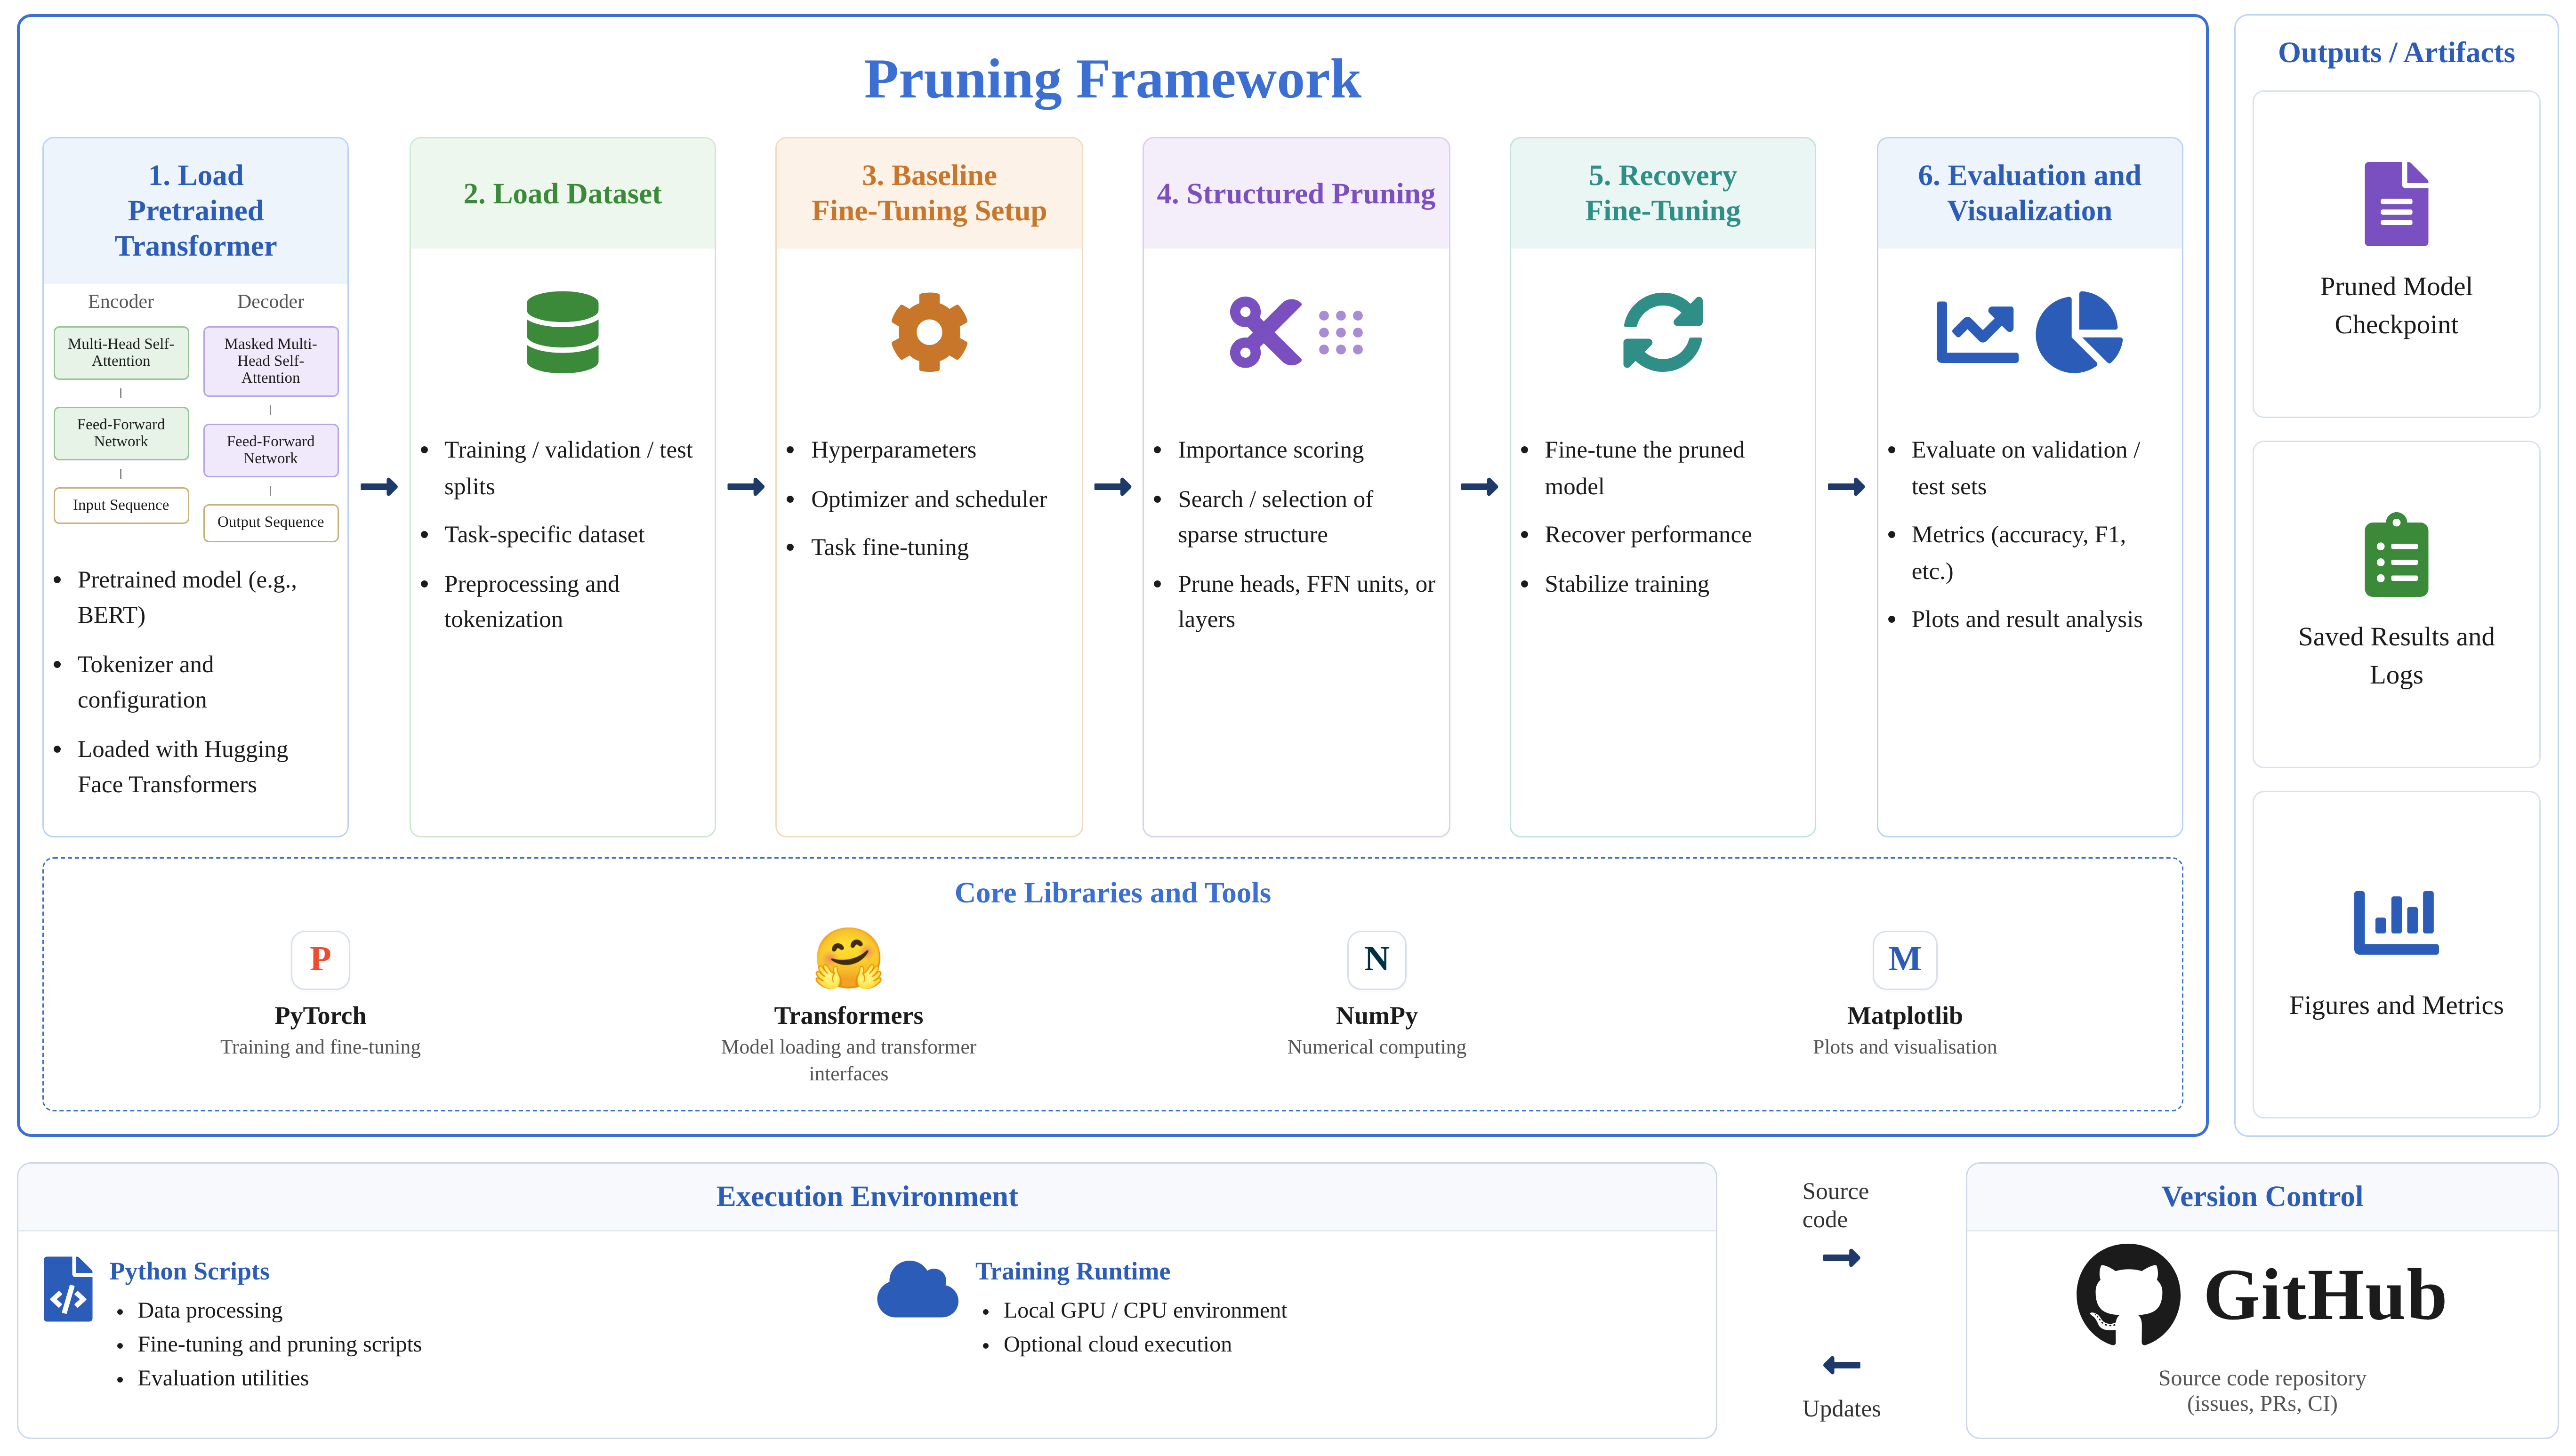
\includegraphics[width=1.3\textwidth,height=0.7\textheight,keepaspectratio]{pipeline.png}%
}
\caption{Technical pipeline of the implemented compression framework. A pretrained Transformer and task dataset are loaded first, a baseline setup fixes the training configuration, the search stage selects a compressed architecture under the active budget constraint, recovery fine-tuning adapts the selected candidate when needed, and the final stage evaluates the model and saves checkpoints, metrics, logs, and figures.}
\label{fig:technical_architecture_pipeline}
\end{figure}

\section{Technologies Used}

This section presents the main technologies used during the design, implementation, experimentation, and management of the proposed solution. These tools provide the required environment for deep learning development, numerical computation, visualization, experiment execution, version control, and project organization.

\subsection{Python}

Python is an open-source, high-level programming language widely used in software development, scientific computing, data analysis, and artificial intelligence. Its ecosystem provides libraries for model implementation, numerical processing, data handling, and experiment automation. The pruning pipeline, training scripts, evaluation scripts, search procedures, and experiment utilities were implemented in Python \cite{pythonAbout,pythonDocs}.

\begin{figure}[H]
	\centering
	
\includegraphics[width=0.35\textwidth]{figures/psf.png}
	\caption{Python logo.}
	\label{fig:python-logo}
\end{figure}

\subsection{Transformers}

Transformers is an open-source library developed by Hugging Face. It provides a unified interface for loading pretrained Transformer models, tokenizers, configuration files, and task-specific model heads \cite{wolf2020transformers,huggingfaceTransformersDocs}.

The implementation uses this library to load the pretrained encoder model and access its internal components. These components include encoder layers, attention modules, feed-forward submodules, hidden states, attention outputs, configuration parameters, and classification heads. Structured pruning requires access to these components because the method removes complete computational units from the model.

Pruning an attention head requires identifying the corresponding projection dimensions inside the attention module. Pruning feed-forward neurons requires selecting intermediate dimensions inside the two-layer feed-forward network. The Transformers library provides a standardized model structure that supports these operations without requiring a complete reimplementation of the architecture.

\begin{figure}[H]
	\centering
	
\includegraphics[width=0.38\textwidth]{figures/transformers.png}
	\caption{Hugging Face Transformers logo.}
	\label{fig:transformers-logo}
\end{figure}

\subsection{PyTorch}

PyTorch is an open-source deep learning framework that provides tensor computation, automatic differentiation, and GPU acceleration. It is commonly used for building, training, and evaluating neural networks. The implementation relies on PyTorch to execute forward passes, compute losses, perform backpropagation, apply masks, update model weights, and run recovery fine-tuning \cite{pytorchDocs,pytorchProject}.

PyTorch is also used to represent pruning masks as tensors. An attention-head mask can be represented as a binary tensor of shape $12 \times 12$ for a model with twelve layers and twelve heads per layer. A feed-forward mask can be represented as a binary tensor of shape $12 \times 3072$ for twelve layers and $3072$ intermediate neurons per layer.

\begin{figure}[H]
	\centering
	
\includegraphics[width=0.35\textwidth]{figures/pytorch.png}
	\caption{PyTorch logo.}
	\label{fig:pytorch-logo}
\end{figure}

\subsection{NumPy}

NumPy is a fundamental Python library for numerical and scientific computing. It provides efficient multidimensional arrays, mathematical operations, random number generation, and linear algebra utilities. NumPy is used for candidate representation, statistical calculations, random sampling, sorting operations, and search-related utilities \cite{numpyOfficial,numpyPyPI}.

Candidate architectures can be stored as arrays indicating the number of active heads and neurons per layer. These arrays are then used to calculate sparsity, compare candidates, and enforce computational constraints.

\begin{figure}[H]
	\centering
	
\includegraphics[width=0.35\textwidth]{figures/numpy_logo.png}
	\caption{NumPy logo.}
	\label{fig:numpy-logo}
\end{figure}

\subsection{Matplotlib}

Matplotlib is a Python library used to create static, animated, and interactive visualizations. It is used to present experimental results, search behavior, pruning statistics, training curves, and comparisons between candidate architectures \cite{matplotlibDocs,matplotlibOfficial}.

Typical visualizations include validation accuracy after recovery, active heads per layer, preserved feed-forward neurons per layer, and the relationship between computational cost and task performance.

\begin{figure}[H]
	\centering
	
\includegraphics[width=0.38\textwidth]{figures/matplotlib.png}
	\caption{Matplotlib logo.}
	\label{fig:matplotlib-logo}
\end{figure}

\subsection{Google Drive}

Google Drive is a cloud storage service that allows files to be uploaded, stored, shared, and accessed from different devices. It is used to organize project files, store experimental outputs, keep backup copies of important resources, and transfer files between working environments \cite{googleDriveOfficial}.

\begin{figure}[H]
	\centering
	
\includegraphics[width=0.34\textwidth]{figures/gd.png}
	\caption{Google Drive logo.}
	\label{fig:google-drive-logo}
\end{figure}

\subsection{Git}

Git is a free and open-source distributed version control system designed to track changes in source code and support collaborative software development. It is used to track modifications to the implementation, preserve experiment scripts, compare previous versions, and maintain a structured development history \cite{gitOfficial,gitBook}.

\begin{figure}[H]
	\centering
	
\includegraphics[width=0.34\textwidth]{figures/git.png}
	\caption{Git logo.}
	\label{fig:git-logo}
\end{figure}

\subsection{GitHub}

GitHub is a cloud-based platform built around Git. It allows developers to store, manage, share, and collaborate on code through repositories. It is used to host the project repository, synchronize code between machines, and maintain a remote copy of the implementation \cite{githubDocs,githubOfficial}.

\begin{figure}[H]
	\centering
	
\includegraphics[width=0.34\textwidth]{figures/github.png}
	\caption{GitHub logo.}
	\label{fig:github-logo}
\end{figure}

\section{Datasets Used}
\label{sec:datasets}

The experimental evaluation uses supervised natural language understanding tasks. These tasks evaluate sentence classification and sentence-pair reasoning after structured pruning.

The selected benchmarks are SST-2, QNLI, and MNLI from the GLUE benchmark \citep{wang2018glue}. The dataset discussion is limited to the required information because the main focus of the project is structured model pruning.

\subsection{Pre-Training Corpora}
\label{subsec:pretraining-corpora}

The pretrained encoder model was originally trained on BooksCorpus and English Wikipedia \citep{devlin2019bert,zhu2015aligning}. BooksCorpus provides long narrative text from unpublished books. English Wikipedia provides factual and encyclopaedic text. These corpora provide broad linguistic representations before supervised task adaptation.

The model uses WordPiece tokenisation \citep{wu2016googles}. Frequent words are represented as complete tokens, while rare words are decomposed into subword units. For example, a rare morphological form can be split into smaller units instead of being mapped to an unknown token. The same tokenizer is preserved during fine-tuning, pruning, and evaluation.

\subsection{Fine-Tuning and Evaluation Benchmarks}
\label{subsec:finetuning-evaluation-benchmarks}

Table~\ref{tab:dataset-examples} presents the selected evaluation tasks, including their input format, label space, and representative labelled examples.

\begin{table}[H]
	\centering
	\scriptsize
	\setlength{\tabcolsep}{3pt}
	\begin{tabularx}{\textwidth}{|>{\raggedright\arraybackslash}p{0.12\textwidth}|X|>{\raggedright\arraybackslash}p{0.24\textwidth}|>{\raggedright\arraybackslash}p{0.16\textwidth}|}
		\hline
		\textbf{Task} & \textbf{Example Input} & \textbf{Possible Labels} & \textbf{Correct Label} \\
		\hline
		SST-2 &
		Sentence: \textit{``The movie is beautifully acted and emotionally powerful.''} &
		\texttt{positive}, \texttt{negative} &
		\texttt{positive} \\
		\hline
		SST-2 &
		Sentence: \textit{``The story is dull, slow, and completely forgettable.''} &
		\texttt{positive}, \texttt{negative} &
		\texttt{negative} \\
		\hline
		QNLI &
		Question: \textit{``Where is the Eiffel Tower located?''}
		
		Sentence: \textit{``The Eiffel Tower is located in Paris, France.''} &
		\texttt{entailment}, \texttt{not\_entailment} &
		\texttt{entailment} \\
		\hline
		QNLI &
		Question: \textit{``Where is the Eiffel Tower located?''}
		
		Sentence: \textit{``The Eiffel Tower was completed in 1889.''} &
		\texttt{entailment}, \texttt{not\_entailment} &
		\texttt{not\_entailment} \\
		\hline
		MNLI &
		Premise: \textit{``A man is playing a guitar on stage.''}
		
		Hypothesis: \textit{``A person is performing music.''} &
		\texttt{entailment}, \texttt{contradiction}, \texttt{neutral} &
		\texttt{entailment} \\
		\hline
		MNLI &
		Premise: \textit{``A man is playing a guitar on stage.''}
		
		Hypothesis: \textit{``No one is playing an instrument.''} &
		\texttt{entailment}, \texttt{contradiction}, \texttt{neutral} &
		\texttt{contradiction} \\
		\hline
		MNLI &
		Premise: \textit{``A man is playing a guitar on stage.''}
		
		Hypothesis: \textit{``The man is performing in a crowded theatre.''} &
		\texttt{entailment}, \texttt{contradiction}, \texttt{neutral} &
		\texttt{neutral} \\
		\hline
	\end{tabularx}
	\caption{Input formats and label spaces for the selected evaluation tasks.}
	\label{tab:dataset-examples}
\end{table}

\subsubsection{SST-2}
\label{subsubsec:sst2}

SST-2 is a binary sentiment classification task derived from the Stanford Sentiment Treebank \citep{socher2013recursive}. Each input is a single sentence, and the model predicts whether its sentiment is \texttt{positive} or \texttt{negative}.

This task provides a sentence-level evaluation of the compressed model. A model must distinguish positive expressions such as \textit{``excellent and moving''} from negative expressions such as \textit{``boring and weak''}. Accuracy is used as the evaluation metric.

\subsubsection{QNLI}
\label{subsubsec:qnli}

QNLI is derived from the Stanford Question Answering Dataset \citep{rajpurkar2016squad}. It is formulated as a sentence-pair classification task. The input contains a question and a candidate sentence. The model predicts one of two labels: \texttt{entailment} or \texttt{not\_entailment}.

A label of \texttt{entailment} indicates that the sentence contains the answer to the question. A label of \texttt{not\_entailment} indicates that the sentence does not provide the requested information. For example, if the question asks where the Eiffel Tower is located, the sentence \textit{``The Eiffel Tower is located in Paris, France''} receives the label \texttt{entailment}. The sentence \textit{``The Eiffel Tower was completed in 1889''} receives the label \texttt{not\_entailment}.

This task evaluates the ability of the compressed model to compare two text segments. Accuracy is used as the evaluation metric.

\subsubsection{MNLI}
\label{subsubsec:mnli}

MNLI is a natural language inference task \citep{williams2018broad}. Each input contains a premise and a hypothesis. The model predicts one of three labels: \texttt{entailment}, \texttt{contradiction}, or \texttt{neutral}.

A label of \texttt{entailment} indicates that the hypothesis follows from the premise. A label of \texttt{contradiction} indicates that the hypothesis is incompatible with the premise. A label of \texttt{neutral} indicates that the hypothesis may be possible without being guaranteed by the premise.

For example, given the premise \textit{``A man is playing a guitar on stage''}, the hypothesis \textit{``A person is performing music''} receives the label \texttt{entailment}. The hypothesis \textit{``No one is playing an instrument''} receives the label \texttt{contradiction}. The hypothesis \textit{``The man is performing in a crowded theatre''} receives the label \texttt{neutral}, since the premise does not specify the audience or the exact venue.

MNLI provides a stronger sentence-pair reasoning evaluation than single-sentence sentiment classification. Accuracy is used as the reported metric.

\subsection{Language Model Evaluation Datasets}
\label{subsec:lm-datasets}

The language model pruning experiments use three standard perplexity benchmarks to evaluate the compressed models.

\subsubsection{WikiText-2}
WikiText-2 is a word-level language modelling benchmark derived from verified Good and Featured Wikipedia articles \citep{merity2017pointer}. It provides a clean, coherent corpus of encyclopaedic text. Perplexity on the test split is the standard evaluation metric; lower values indicate better language modelling quality.

\subsubsection{C4}
C4 (Colossal Clean Crawled Corpus) is a large-scale web text corpus produced by applying aggressive filtering and deduplication to Common Crawl snapshots \citep{raffel2020exploring}. It covers a broad range of domains and writing styles and is commonly used both as a pretraining source and as an out-of-domain perplexity benchmark for evaluating generalisation after compression.

\subsubsection{FineWeb-Edu}
FineWeb-Edu is a high-quality subset of the FineWeb web corpus filtered for educational content \citep{lozhkov2024fineweb_edu}. The filtering pipeline uses a classifier trained to identify instructional and informative text. It provides a more domain-specific evaluation signal than general web corpora and has been adopted as a benchmark for assessing language model quality on structured, factual text.

\section{Model}
\label{sec:models}

\subsection{BERT}
\label{subsec:bert}

BERT is an encoder-only Transformer architecture trained with masked language modelling and next-sentence prediction \citep{devlin2019bert,vaswani2017attention}. Its bidirectional self-attention allows each token representation to incorporate information from both left and right context.

BERT\textsubscript{BASE} contains twelve Transformer encoder layers. Each layer has twelve attention heads and a feed-forward block with intermediate width $3072$. The hidden size is $768$, and the full model contains approximately $110$ million parameters. For classification tasks, the representation of the \texttt{[CLS]} token is passed to a task-specific classifier.

The pruning procedure targets structured units inside the encoder blocks. Attention heads and feed-forward neurons are removed as complete units. This pruning form supports practical acceleration because it can reduce matrix dimensions and remove complete computational paths.

For example, if layer $3$ preserves only $2$ attention heads out of $12$, then the attention computation in that layer is reduced. If the same layer preserves only $192$ feed-forward neurons out of $3072$, then the intermediate feed-forward projection is also reduced. The final compressed architecture is therefore described by its total sparsity and by the distribution of preserved units across layers.

\subsection{EleutherAI Pythia-1.4B}
\label{subsec:pythia}

Pythia is a suite of autoregressive decoder-only language models released by EleutherAI and trained on The Pile, a diverse 825\,GB English text corpus \citep{biderman2023pythia}. The suite spans eight model sizes from 70M to 12B parameters and was designed to support reproducible research on scaling laws, training dynamics, and model analysis.

Pythia-1.4B contains 24 Transformer decoder layers with a hidden dimension of 2048, 16 attention heads per layer, and a feed-forward intermediate width of 8192. The model has approximately 1.4 billion parameters. It uses rotary position embeddings and parallel attention and feed-forward computation within each layer.

This model is selected for the language model pruning experiments because its size is tractable for iterative search-based compression on a single GPU, while being large enough to exhibit realistic structured redundancy across layers. Perplexity on WikiText-2, C4, and FineWeb-Edu is used as the evaluation metric.

\section{Experimental Environment}
\label{sec:experimental-environment}

All experiments are conducted on a laptop equipped with an NVIDIA RTX 4090 Laptop GPU with 16\,GB of VRAM. Model loading, tokenization, fine-tuning, pruning, checkpoint handling, and evaluation are implemented using the Hugging Face Transformers library \citep{wolf2020transformers}.

Mixed precision training is used when numerically stable \citep{micikevicius2018mixed}. It reduces memory consumption and can improve throughput on compatible hardware. Numerical stability is monitored during recovery fine-tuning, especially for highly compressed architectures.

The hardware environment imposes practical constraints on the experimental protocol. Laptop GPUs are affected by thermal limits, power configuration, driver behavior, and cooling conditions. Therefore, wall-clock measurements are hardware-dependent. Small accuracy differences are interpreted cautiously because repeated runs may vary due to random initialization, data ordering, dropout, and GPU-level nondeterminism.

\subsection{Baselines and Reporting}

Included in the comparison is our search approach and random, beam search and structured pruning comparisons, drawing structured pruning refs from CoFi \citep{xia2022cofi} and ZipLM \citep{kurtic2023ziplm}. Comparisons are made at the same constraints where possible, particularly the target computation budget, recovery process and measure.

For the decoder-model searches on Pythia-1.4B (layer drop, quant and low-rank factorisation), we compare against EvoPress \citep{evopress2024}, a search-based approach whose evolutionary algorithm and KL-divergence fitness are most similar to our approach. Both methods are run at the same sparsity or bit-width target and compared over the same perplexity datasets.

\subsection{Level Database and Token Budgets}

Both the quantization and the low-rank search are performed on a level database that has been generated beforehand. For each weight matrix, weights are pre-compressed to every possible level and persisted to disk: one GPTQ-quantized copy at each bit-width, and a truncated-SVD factor pair at each rank (plus the residue singular triplets required to recover weights). During search, each candidate is assembled by loading the required weights whose names are specified by its per-layer level vector. No decompression or on-the-fly compression happens and each query takes one forward pass.

Each of the searches tunes to approximately 250,000 held-out tokens. This is well below the budgets spent by the bigger baseline models, and necessary given the 16 GB of VRAM on the GPU. Candidates are scored using the multi-stage process described in Section~\ref{chap:ga} above: the early stages screen the population efficiently by spending a limited number of tokens per candidate, and the remaining candidates are then scored on more tokens to make the selection. Final perplexity is reported over the entire test sets.
% !TEX root = ../../main_without_quantization.tex
\section{Conclusion}
\label{chap:methodology_conclusion}

In this chapter we have defined the entire implementation pipeline that is utilized for this work. Initially, we parameterize the compressed architecture in binary structural parameters, after which we constrain the candidate space using a cost budget based model for both the encoder and the decoder. We then compare candidate masks prior to recovery, using a calibration based surrogate metric; we finally find the mask using a genetic search, with efforts to keep variety within the different architectural regions of the candidate space, and recover the final architecture using cascaded distillation, using the already found mask.

The primary design decision here is the distinction between architecture selection and parameter recovery. The search stage determines where the rest of the computation is assigned; and the recovery stage would fine tune only the selected architectures' surviving parameters.

The next chapter reports the observed performance of the selected models and compares the proposed search procedure with other search baselines and well know pruning methods from the literature.


\chapter{Results}

% !TEX root = ../../main_without_quantization.tex
This Chapter reports two groups of results under the experimental setting of Section~\ref{sec:experimental-environment}. The first group evaluates encoder-side structured pruning on GLUE classification tasks, where BERT architectures are selected by search and then recovered with the distillation procedure of Section~\ref{chap:recovery}. The second group evaluates decoder-side compression on Pythia-1.4B, where perplexity replaces accuracy and the same search machinery is applied to layer sparsity, low-rank factorization, and quantization.

\section{Result Tables and Discussion}
\label{chap:results}



Table~\ref{tab:key_results} summarizes the main empirical takeaways before the detailed comparisons. The table is intentionally selective: it highlights the strongest size-matched or near-size results without replacing the full task tables.

\begin{table}[H]
\centering
\scriptsize
\setlength{\tabcolsep}{4pt}
\renewcommand{\arraystretch}{1.08}
\caption{Selected headline results. Accuracy is higher-is-better for GLUE; perplexity is lower-is-better for Pythia-1.4B.}
\label{tab:key_results}
\begin{tabularx}{\textwidth}{@{}p{0.25\textwidth}X@{}}
\toprule
Setting & Result \\
\midrule
SST-2, 7.0M & Ours 93.35 vs ZipLM 93.0 at 5.7M and CoFi 91.51 \\
SST-2, 4.0M & Ours 92.43 vs ZipLM 91.7 at 4.2M \\
QNLI, 3.0M & Ours 88.2 vs ZipLM 87.6 at 3.2M \\
Low-rank FT, WikiText-2 & Ours 24.91 vs EvoPress 28.656 \\
Quantization, 2.5 bits & EvoPress 33.06 vs ours 33.19 on WikiText-2 \\
\bottomrule
\end{tabularx}
\end{table}

In addition to accuracy, the procedure has a measurable runtime cost. Under the hardware setting of Section~\ref{sec:experimental-environment}, end-to-end runs on QNLI and SST-2 required nearly six hours on average, whereas MNLI required about thirty hours on average. This difference is consistent with the larger training split and heavier recovery cost of MNLI.

\subsection{Encoder Classification Results}
\label{subsec:encoder-results}

\subsubsection{Search Baselines}

The first question is whether the evolutionary search improves on simpler budget-constrained selection rules. Table~\ref{tab:search_baselines} compares the proposed method against random search and beam search under matched recovery and matched budget targets. The comparison is organised by the final recovered model size, since the search problem changes materially between the tiny and moderate regimes.

\begin{table}[H]
\centering
\scriptsize
\setlength{\tabcolsep}{4pt}
\renewcommand{\arraystretch}{1.08}
\caption{Development accuracy under matched recovery for three search strategies. Random search and beam search use the same teacher, budget band, and recovery procedure as the proposed method.}
\label{tab:search_baselines}
\begin{tabular}{llcccc}
\toprule
Task & Final model & Params & Random & Beam & Ours \\
\midrule
QNLI  & tiny      & 3.0M  & 84.72 & 85.36 & \textbf{88.20} \\
QNLI  & moderate  & 34.1M & 90.74 & 91.10 & \textbf{91.90} \\
MNLI  & tiny      & 3.1M  & 80.18 & 80.76 & \textbf{81.34} \\
MNLI  & moderate  & 34.0M & 84.92 & 85.19 & \textbf{85.60} \\
SST-2 & tiny      & 3.3M  & 91.21 & 91.76 & \textbf{92.43} \\
SST-2 & moderate  & 39.0M & 93.08 & 93.31 & \textbf{93.70} \\
\bottomrule
\end{tabular}
\end{table}

The margin is maximal at the very small end. At 3.0 M on QNLI, our search returns 88.2 while beam search gets 85.36 and random search is lower still. This is repeated on MNLI and SST-2; in the very small regime where budget constrains the search to that architecture size, recoverability is directly correlated with the quality of search. The range decreases as we move into the moderate regime where our search still remains ahead. This is in line with our design choice; in the cases where many viable candidates share equal costs, random search and beam search still find viable masks, but do not maintain the structural diversity that island-based evolution preserves.

\subsubsection{Comparison to Structured Pruning Baselines}

The second question is whether the recovered models remain competitive against established structured pruning methods at comparable sizes. Table~\ref{tab:literature_comparison} compares the recovered models against representative CoFi and ZipLM results, together with the task-fine-tuned uncompressed baseline used in this study.

\begin{table}[H]
\centering
\scriptsize
\setlength{\tabcolsep}{4pt}
\renewcommand{\arraystretch}{1.08}
\caption{Comparison against structured pruning baselines and the uncompressed task baseline. Scores are development accuracy.}
\label{tab:literature_comparison}
\begin{tabular}{llrrl}
\toprule
Task & Model & Params & Score & Note \\
\midrule
\multirow{7}{*}{QNLI}
& CoFi, 95\% & 5.0M  & 86.1  & high compression \\
& ZipLM, near-size & 3.2M  & 87.6  & $13\times$ speedup \\
& \textbf{Ours} & \textbf{3.0M}  & \textbf{88.2}  & best tiny model \\
& CoFi, 60\% & 34.0M & 91.8  & moderate compression \\
& ZipLM, $2\times$ & 38.0M & 91.4  & near-size reference \\
& \textbf{Ours} & \textbf{34.1M} & \textbf{91.9}  & above baseline \\
& task baseline & full  & 91.4  & uncompressed run \\
\midrule
\multirow{7}{*}{MNLI}
& CoFi, 95\% & 5.0M  & 80.6  & high compression \\
& ZipLM, near-size & 3.5M  & 81.3  & $13\times$ speedup \\
& \textbf{Ours} & \textbf{3.1M}  & \textbf{81.34}  & above near-size baseline \\
& CoFi, 60\% & 34.0M & 85.3  & moderate compression \\
& ZipLM, $2\times$ & 38.5M & 84.8  & close size \\
& \textbf{Ours} & \textbf{34.0M} & \textbf{85.6}  & above both \\
& task baseline & full  & 84.7  & uncompressed run \\
\midrule
\multirow{15}{*}{SST-2}
& CoFi, compact & 4.4M  & 91.1  & near tiny-size comparison \\
& ZipLM, compact & 4.2M  & 91.7  & near-size comparison \\
& \textbf{Ours} & \textbf{4.0M}  & \textbf{92.43} & above near-size ZipLM \\
& ZipLM, compact & 3.6M  & 91.7  & same size as ours \\
& \textbf{Ours} & \textbf{3.6M}  & 91.6 & above CoFi, near ZipLM \\
& CoFi, 90\% sparse & $\approx$8.5M & 91.51 & $0.1 \times 85$M encoder \\
& ZipLM, compact & 5.7M  & 93.0  & compact reference \\
& \textbf{Ours} & \textbf{7.0M}  & \textbf{93.35} & above CoFi and compact ZipLM \\
& CoFi, 95\% & 5.0M  & 90.4  & high compression \\
& ZipLM, near-size & 3.6M  & 91.7  & $14\times$ speedup \\
& \textbf{Ours} & \textbf{3.3M}  & \textbf{92.43} & strongest earlier tiny run \\
& CoFi, 60\% & 34.0M & 93.0  & moderate compression \\
& ZipLM, $2\times$ & 38.7M & 93.4  & close size \\
& \textbf{Ours} & \textbf{39.0M} & \textbf{93.7}  & best moderate model \\
& task baseline & full  & 93.22 & uncompressed run \\
\bottomrule
\end{tabular}
\end{table}
We make three general observations from these results. First, our technique is  most promising in the small-model regime. The gaps with CoFi and ZipLM are greatest between $3$M and $7$M parameters; at this point, the other part of the architecture has little room for capacity. Specifically, our $7.0$M model for SST-2 performs at $93.35$ while the best compact result for CoFi is $91.51$ and ZipLM performs at $93.0$ at $5.7$M parameters. Our $4.0$M model is at $92.43$ compared to $91.7$ for ZipLM at $4.2$M, and our $3.6$M model is at $91.6$, greater than the $4.4$M CoFi model and similar to the $3.6$M ZipLM model. For the $90\%$ sparse CoFi result, the estimated size of the encoder remaining is approximately $8.5$M parameters, because the encoder that was reported had approximately $85$M parameters. Second, the moderate-compression results also perform competitively. The QNLI model of $34.1$M parameters achieves $91.9$, our MNLI model of $34$M parameters achieves $85.6$, and our SST-2 model of $39$M parameters achieves $93.7$. Third, the recovered models do approach the baseline performance at the corresponding task. The differences are minimal at QNLI and SST-2 and compare favorably to the stated results at similar sized networks. This means our search has value beyond finding the desired compression ratio, in that we can search for compressible architecture that may perform well even after pruning.
\subsection{Decoder Compression Results (Pythia-1.4B)}
\label{subsec:lm-results}

\subsubsection{Layer-Sparsity Search}

The decoder experiments probe if the same genetic search machinery generalize to things outside of encoder pruning so it transcends into a generic framework. In these the candidate is a decoder compression scheme applied to Pythia-1.4B, and the candidates are evaluated by their perplexity on WikiText-2, C4, and FineWeb-Edu. EvoPress [evopress2024] is the closest baseline because it searches with evolutionary algorithms and it scores candidates using KL divergence similar to ours. The baselines are tested with identical sparsity values and identical datasets to the ones in this paper.

Table~\ref{tab:lm-25-sparsity} reports results at $25\%$ sparsity. The proposed method reaches lower perplexity than EvoPress on all three datasets after only 11 generations, whereas EvoPress requires 72 generations to reach its reported values. This earlier convergence reflects the efficiency of the search procedure in identifying well-structured sparse configurations under tight generation budgets.

\begin{table}[H]
\centering
\caption{Perplexity ($\downarrow$) on Pythia-1.4B at $25\%$ sparsity. EvoPress results are reported at generation 72; ours at generation 11.}
\label{tab:lm-25-sparsity}
\begin{tabular}{lcc}
  \toprule
  \textbf{Dataset} & \textbf{EvoPress (gen 72)} & \textbf{Ours (gen 11)} \\
  \midrule
  FineWeb-Edu & 25.69 & \textbf{23.58} \\
  WikiText-2  & 28.38 & \textbf{25.00} \\
  C4          & 31.36 & \textbf{28.66} \\
  \bottomrule
\end{tabular}
\end{table}

Table~\ref{tab:lm-50-sparsity} reports results at $50\%$ sparsity, a significantly more aggressive compression target, under the larger $2$M-token calibration setting for both methods. At this regime, EvoPress reaches perplexity values of $152.50$, $208.50$, and $184.00$ on FineWeb-Edu, WikiText-2, and C4 respectively after 90 generations. The proposed method achieves lower perplexity on all three datasets after only 30 generations, demonstrating that the search is effective even under severe compression where maintaining language model coherence is substantially harder.

\begin{table}[H]
\centering
\caption{Perplexity ($\downarrow$) on Pythia-1.4B at $50\%$ sparsity. EvoPress results are reported at generation 90; ours at generation 30.}
\label{tab:lm-50-sparsity}
\begin{tabular}{lcc}
  \toprule
  \textbf{Dataset} & \textbf{EvoPress (gen 90)} & \textbf{Ours (gen 30)} \\
  \midrule
  FineWeb-Edu & 152.50 & \textbf{131.00} \\
  WikiText-2  & 208.50 & \textbf{155.50} \\
  C4          & 184.00 & \textbf{159.88} \\
  \bottomrule
\end{tabular}
\end{table}

We also evaluated a separate $50\%$ layer-sparsity setting using a smaller calibration budget of approximately $131$k tokens for both methods. This lower-calibration run is therefore kept separate from the headline $2$M-token comparison, but it is still informative: under the smaller calibration budget, the proposed configuration remains below EvoPress on all three evaluation datasets.

\begin{table}[H]
\centering
\caption{Additional $50\%$ layer-sparsity result under a lower calibration budget for both methods. Perplexity is lower-is-better.}
\label{tab:lm-50-sparsity-lowcalib}
\begin{tabular}{lcc}
  \toprule
  \textbf{Dataset} & \textbf{EvoPress (131k tokens)} & \textbf{Ours (131k tokens)} \\
  \midrule
  FineWeb-Edu & 154.88 & \textbf{132.500} \\
  WikiText-2  & 202.12 & \textbf{195.875} \\
  C4          & 189.88 & \textbf{168.875} \\
  \bottomrule
\end{tabular}
\end{table}

Proposed method achieves better perplexity compared to EvoPress with less generation counts in both sparsity levels. At 50\% sparsity, the perplexity difference is above 50 for WikiText-2, and over 20 for FineWeb-Edu and C4. We can conclude that evolutionary search also transfer well to generative language models as measured by perplexity and it is not just the performance gained for encoder-based classification models.

\subsubsection{Low-Rank Factorization}
\label{subsec:lm-lowrank}

Table~\ref{tab:lm-lowrank} reports perplexity results when the search is applied to low-rank factorization on Pythia-1.4B. The baseline is EvoPress. The proposed method reaches lower perplexity on all three evaluation datasets.

\begin{table}[H]
\centering
\caption{Perplexity ($\downarrow$) on Pythia-1.4B under low-rank factorization. EvoPress is the baseline.}
\label{tab:lm-lowrank}
\begin{tabular}{lcc}
  \toprule
  \textbf{Dataset} & \textbf{EvoPress} & \textbf{Ours} \\
  \midrule
  FineWeb-Edu & 63.34 & \textbf{59.97} \\
  WikiText-2  & 33.50 & \textbf{29.65} \\
  C4          & 83.88 & \textbf{80.94} \\
  \bottomrule
\end{tabular}
\end{table}

The second low-rank table evaluates the recovery fine-tuning stage applied after search. This stage is part of the recovery pipeline rather than a new search objective: the architecture is fixed, and the remaining step adapts the selected low-rank model. It improves both methods, but the proposed search still retains a clear advantage after fine-tuning.

\begin{table}[H]
\centering
\caption{Perplexity ($\downarrow$) on Pythia-1.4B under low-rank factorization, after recovery fine-tuning.}
\label{tab:lm-lowrank-ft}
\begin{tabular}{lcc}
  \toprule
  \textbf{Dataset} & \textbf{EvoPress} & \textbf{Ours} \\
  \midrule
  FineWeb-Edu & 53.219 & \textbf{46.25} \\
  WikiText-2  & 28.656 & \textbf{24.91} \\
  C4          & 68.500 & \textbf{64.06} \\
  \bottomrule
\end{tabular}
\end{table}

The fine-tuned low-rank results show the effect of the selected rank allocation after recovery. EvoPress uses the same recovery stage, so both methods benefit from fine-tuning. After the stage, the proposed model remains lower by $6.969$ perplexity on FineWeb-Edu, $3.746$ on WikiText-2, and $4.440$ on C4.

\subsubsection{Quantization}
\label{subsec:lm-quant}

Tables~\ref{tab:lm-quant-225} and~\ref{tab:lm-quant-25} report perplexity results under post-training quantization at two average bit-widths. The baseline is EvoPress.

\begin{table}[H]
\centering
\caption{Perplexity ($\downarrow$) on Pythia-1.4B at $2.25$ bits average quantization.}
\label{tab:lm-quant-225}
\begin{tabular}{lcc}
  \toprule
  \textbf{Dataset} & \textbf{EvoPress} & \textbf{Ours} \\
  \midrule
  FineWeb-Edu & 45.97  & \textbf{45.63} \\
  WikiText-2  & 81.00  & \textbf{76.69} \\
  C4          & 65.06  & \textbf{63.84} \\
  \bottomrule
\end{tabular}
\end{table}

At $2.25$ bits, the proposed method reaches lower perplexity than EvoPress on all three datasets, with the most visible gap on WikiText-2.

\begin{table}[H]
\centering
\caption{Perplexity ($\downarrow$) on Pythia-1.4B at $2.5$ bits average quantization.}
\label{tab:lm-quant-25}
\begin{tabular}{lcc}
  \toprule
  \textbf{Dataset} & \textbf{EvoPress} & \textbf{Ours} \\
  \midrule
  FineWeb-Edu & \textbf{25.14} & 25.80 \\
  WikiText-2  & \textbf{33.06} & 33.19 \\
  C4          & \textbf{32.84} & 33.69 \\
  \bottomrule
\end{tabular}
\end{table}

At $2.5$ bits, EvoPress holds a small edge on all three datasets, with gaps below one perplexity point. Results at this bit-width are competitive across both methods. This is a useful boundary case: the search is not presented as uniformly dominating EvoPress, but as competitive when the compression level changes.

% !TEX root = ../../main_without_quantization.tex
\section{Conclusion}
\label{chap:results_conclusion}

This chapter tested the proposed search framework on encoder-side structured pruning and decoder-side compression. As for the encoder experiment, we can find that the search is most meaningful when the reduced architecture is extremely small, where the assignment of heads and feed-forward capacity is critical for recovery. In the decoder experiments, the same search principle holds outside of pruning. We demonstrate notable improvement for layer sparsity and low-rank factorization, and competitive performance in the quantization scenario.

From this follows our findings provide empirical support for the core hypothesis of the paper: rather than individual local decisions, it is better to view compressed Transformers as holistic architectures optimized within a given budget. The primary challenge remains the overhead from search and recovery; however, as illustrated, this cost can often be justified by the search for aggressively compressed but recoverable architectures.
